\chapter{Design}
\label{chapter:design}

In this chapter, we lay out the requirements that an implementation of a WebAssembly container runtime should satisfy in general. We introduce several WebAssembly runtimes and pick three of them for our implementation. We then expand on the requirements by looking at OpenWhisk specifically and how we need to modify it to enable our new container runtime, but also detail other approaches that could be used to run WebAssembly workloads. Finally, we describe and discuss our concrete implementation in Apache OpenWhisk, how to achieve fast cold starts and high performance, while also examining the trade-offs involved.

\section{Core approach}

As we've seen in the previous chapter, there are a number of issues with serverless in general, but also serverless on the edge. In this section we will summarize the core problem and describe our idea for rectifying these issues to make serverless (edge) computing more viable.

A substantial cold start latency has emerged as the paramount issue of the serverless platform. It prevents serverless platforms from implementing true scale-to-zero, since functions are kept warm after invocations, wasting energy and resources. While we may not be able to get rid of the keep-alive completely, a significant reduction in cold start latency would allow a similarly large reduction in keep-alive time. Since energy and resources are even more precious on typical edge devices, this is also very important for their quality of service.
Average cold start times are on the same order of magnitude as average function execution times, thereby significantly impacting the quality of service a serverless platform can offer. Moreover, serverless is employed by developers for bursty, unpredictable workloads, a pattern that is also common at the edge. In this scenario we see concurrent requests, which translate to concurrent cold starts. The more concurrent cold starts, the longer each one takes \cite{Cui2018}.
Operators are forced to choose between saving cost and resources or enabling a high quality of service -- in particular shorter response times. While this trade-off is inevitable to some degree, the cold start exacerbates it. A new container runtime must alleviate that latency, to provide mutual benefits for the serverless user and the operator.

Serverless enables the execution of »polyglot tenant-provided code« \cite{Nastic2018}. A new runtime must keep up these principles of being programming language agnostic to continue enabling all developers to use the serverless platform.
To allow for multi-tenancy on the same physical host, containers need to be sandboxed securely. As described in the previous chapter, WebAssembly provides sandboxing and support for many languages, with support for more likely to come. At the same time, it is a lighter-weight solution than virtualization with Docker containers. In contrast to Docker, its isolation does not depend on operating system features, which may incurr a performance cost on the downside. Thus, it seems like a good candidate to replace Docker containers in serverless platforms while alleviating the cold start latency. This is also why WebAssembly may fare better on low-power edge devices.

\citeauthor{Mendki2020} compared WebAssembly and Docker container startup times, and found WebAssembly being 91\% faster than containers and used 75\% less memory \cite{Mendki2020}. \citeauthor{Hall2019} found their WebAssembly-based serverless platform fared 60\% better, on average, than the Docker container solution, for their concurrent »Multiple Client, Multiple Access« workload \cite{Hall2019}. These promising results are the basis for our work and validate the core idea of the approach.

\section{Requirements}

Some of the requirements for a WebAssembly container runtime are a direct consequence of the issues we have assessed. We will expand on others in the following sections. The summary of concerns and requirements are:

\begin{enumerate}
    \item Be easily integratable with an existing serverless framework.
    \item Be programming-language agnostic.
    \item Provide a cheap sandboxing mechanism to ensure multi-tenant capability and no adverse effects on the cold start latency.
    \item Be as close to native speed as possible to be a viable alternative to existing container runtimes.
    \item Run on devices with potentially different instruction set architectures (at least \inl{x86\_64} and \inl{ARM}).
    \item Be able to efficiently handle a large amount of I/O concurrently, due to all requests being proxied through.
    \item Be thread-safe.
\end{enumerate}

Finding a suitable serverless framework that we can modify and integrate with, will be the topic of the next section. In chapter \ref{chapter:background} and the preceding section we have seen how WebAssembly provides some of these requirements, such as sandboxing, good execution speed and language-agnosticism. However, for our implementation we need concrete WebAssembly runtimes that provide these properties, so we will explore the options for such runtimes and work out the differences. The choice for which language and libraries to implement our executor with will be driven by how the Wasm runtimes we choose can be integrated. Other concerns include having access to highly performant, concurrent I/O and support for correctness guarantees, including thread-safety.

\subsection{Apache OpenWhisk}

We use Apache OpenWhisk as the framework to implement WebAssembly support for. OpenWhisk is a production-ready framework, used as the basis for IBM's Cloud Functions. Thus, implementing Wasm support in OpenWhisk would show the viability of the approach in the real world. The framework is also frequently used by serverless researchers to implement new ideas such as pause containers to reduce cold start times \cite{Mohan2019} or Wasm support via \inl{node.js} \cite{Hall2019}, making it a well-respected and frequently used framework. OpenWhisk also has \emph{lean} components, which are lighter-weight replacements for its heavier ones, such as Kafka. These enable OpenWhisk to be deployed on edge devices, such as Raspberry Pis, on which we plan to evaluate our implementation. Furthermore, because OpenWhisk is already designed to be easily extensible with new language runtimes, the protocol is straightforward to implement.

\section{WebAssembly runtimes}
\label{section:wasm-runtimes}

WebAssembly is a specification\footnote{\url{https://webassembly.org/specs/}} and implementations adhering to this specification are WebAssembly runtimes. Since Wasm was originally designed for the web, the virtual machines of browsers, such as Google's V8 or Mozilla's SpiderMonkey, can also execute WebAssembly in addition to JavaScript. With the rise of Wasm outside the Web, a large number of standalone runtimes have emerged and many are actively being developed. This section will introduce a number of runtimes with different execution models, and justify our choice of runtimes to implement in our executor.


\subsection{Wasmtime}

Wasmtime\footnote{\url{https://github.com/bytecodealliance/wasmtime}} is a runtime that has support for Just-in-Time compilation, available for the x86\_64 and aarch64 instruction set architectures (ISA). It is written in Rust and thus easily embeddable from there. Support for the latest WASI standards and future proposals for Wasm are implemented.
It is developed as part of the Bytecode Alliance\footnote{\url{https://bytecodealliance.org/}}, with founding members like Mozilla, fastly, Intel and RedHat. The \inl{cranelift} code generator is developed as part of the alliance and \inl{wasmtime} uses it for Just-in-Time compilation. The code generator's documentation points out that the backend for \inl{x86\_64} is »the most complete and stable; other architectures are in various stages of development \cite{Alliance2021}.« 
Thus it will most likely run on an \inl{aarch64} Raspberry Pi, but performance may not be on-par with an \inl{LLVM}-based runtime.

\subsection{Lucet}

Lucet\footnote{\url{https://github.com/bytecodealliance/lucet}} is the compiler and runtime used for cloud provider fastly's Terrarium, a platform for running WebAssembly on edge devices \cite{fastly2019}. It consists of a compiler and a runtime to execute WebAssembly. The compiler, \inl{lucetc}, compiles Wasm modules to native object or shared object files. The complementary \inl{lucet-runtime} can then load the native code and call the contained Wasm functions. Because of this compilation model, execution can reach near-native speeds. However, the execution is not sandboxed by default, requiring mechanisms like \inl{seccomp-bpf}\footnote{\url{https://wiki.mozilla.org/Security/Sandbox/Seccomp}}, and the security model is actively being developed. It is currently only available on the \inl{x86\_64} ISA. Since we require support for edge devices, typically built on the arm ISA, we will not be using \inl{lucet}. Furthermore, the lack of mature sandboxing makes other runtimes a better choice.

\subsection{Wasmer}

Wasmer\footnote{\url{https://github.com/wasmerio/wasmer}} is a WebAssembly runtime with support for the three major platforms and \inl{x86\_64} and \inl{aarch64} ISAs. Notably, wasmer has already reached version \inl{1.0}, indicating a certain level of maturity. The runtime offers three different compilers, \inl{singlepass}, \inl{cranelift} and \inl{LLVM}, whose compilation times get slower and execution times get faster, in that order, respectively. The runtime has a JIT and a native engine, which differ in the way the module is loaded. In particular, the native engine produces a shared object, which can be loaded with a fast \inl{dlopen} call. The support for high-quality AoT compilation with \inl{LLVM} and fast startup times makes wasmer a promising choice for our purpose.

\subsection{WASM3}

Due to Wasm's simplicity in the binary format, there is wide-spread interest for running it on embedded devices. An example of that is \inl{wasm3}\footnote{\url{https://github.com/wasm3/wasm3}}, a Wasm interpreter that claims to be the fastest. They argue in favor of interpretation over JIT or AoT compilation, since startup latency is more important in many situations. Furthermore, portability and security are easier to achieve with this approach and development with the virtual machine is simpler. Still, a performance penalty of 4 to 5x compared to JIT or 12x compared to native execution, leads us to believe that no amount of startup latency gain can make up for the performance loss. Even though our primary goal is that of reducing the cold start latency, the execution that follows cannot massively lack behind Docker containers, if adoption is to succeed. The relationship between startup and execution performance is too far out of balance in this case.

\subsection{WebAssembly Micro Runtime}

However, there is still value in runtimes written specifically for embedded devices. The WebAssembly Micro Runtime\footnote{\url{https://github.com/bytecodealliance/wasm-micro-runtime/}} (\inl{wamr}) has support for all three mentioned execution modes. It has low memory usage and binary size. For example, the claimed binary size of the AoT runtime is just 50 kilo bytes. Further, the AoT runtime claims near-native speed. For execution on edge devices, where memory is scarce, this runtime may allow more modules to be kept in-memory compared to heaver-weight runtimes.

A summary of the runtimes we looked at can be found in table \ref{table:wasm-runtime-overview}. The diversity of execution modes sticks out -- clearly no single mode is the best for all scenarios. Except for \inl{lucet}, all runtimes have good platform support. However, particularly for edge devices, the lack of support for the 32-bit arm architecture can be challenging in the Rust-written runtimes (\inl{wasmtime}, \inl{wasmer}, \inl{lucet}). The support in the other ones, written in C, is there.

\newcommand{\linux}{\input{icons/linux.pdf_tex}}
\newcommand{\macos}{\input{icons/macos.pdf_tex}}
\newcommand{\windows}{\input{icons/windows.pdf_tex}}
\newcommand{\freebsd}{\input{icons/freebsd.pdf_tex}}
\newcommand{\android}{\input{icons/android.pdf_tex}}
\newcommand{\ios}{\input{icons/ios.pdf_tex}}

\begin{table}[h!]
    \centering
    \begin{tabular}{c | c | c | c}
        Runtime        & ISA support & Execution modes  & Platform support\\
        \hline
        \inl{wasmtime} & \inl{x86\_64}, \inl{aarch64} & AoT, JIT & \linux, \macos, \windows\\
        \inl{lucet}    & \inl{x86\_64} & AoT & \linux, \macos\\
        \inl{wasmer}   & \inl{x86}, \inl{x86\_64}, \inl{aarch64} & AoT, JIT & \linux, \macos, \windows\\
        \inl{wasm3}    & \inl{x86}, \inl{x86\_64}, \inl{arm}, \inl{RISC-V}, ...  & Interpreted      & \linux, \macos, \windows, \freebsd, \android, \ios\\
        \inl{wamr}     & \inl{x86}, \inl{x86\_64}, \inl{arm}, \inl{aarch64}, ... & AoT, Interpreted & \linux, \macos, \windows, \android, ... \\
    \end{tabular}
    \caption{WebAssembly runtime feature overview.}
    \label{table:wasm-runtime-overview}
\end{table}

\section{WebAssembly in OpenWhisk}

In this section we examine the possibilities for bringing WebAssembly support to OpenWhisk.
In the rest of this section we will explore the available options and discuss them in the context of these requirements.

\subsection{OpenWhisk's anatomy}

In order to understand the requirements for our Wasm-flavored OpenWhisk, we need to understand the design of OpenWhisk itself first.

\begin{figure}
    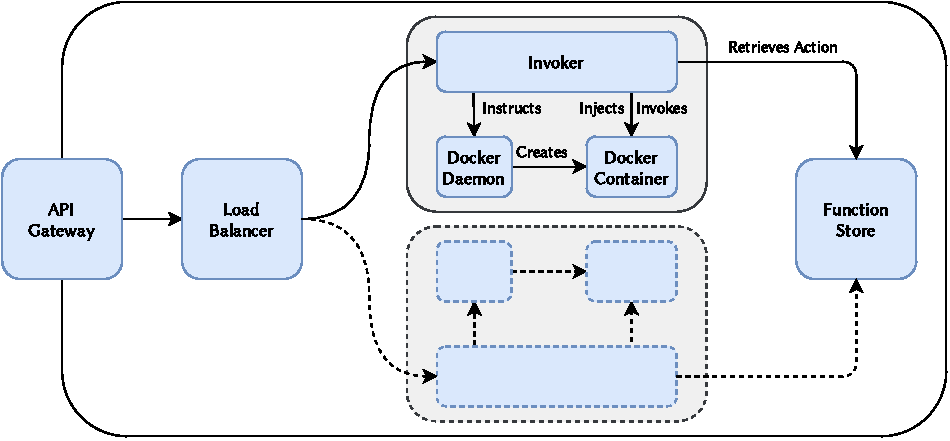
\includegraphics{figures/OpenWhiskActionInvocationFlow.pdf}
    \caption{The invocation flow of an action in Apache OpenWhisk, based on the source code and documentation \cite{OpenWhiskSystemDesign}. Potentially many Invokers can exist on different hosts in this setup.}
    \label{fig:openwhisk-action-invocation-flow}
\end{figure}

Figure \ref{fig:openwhisk-action-invocation-flow} sketches the design of OpenWhisk. Users interact with it through its API Gateway, which consists of \inl{nginx}, mostly for SSL termination, and the \inl{Controller}, which implements the main logic. It handles the creation of actions - OpenWhisk's name for serverless functions - authentication and authorization as well as invoking the action.
In the latter case, the controller uses its load balancer to determine one of the potentially many \inl{Invoker}s, that should handle the request. The \inl{Invoker}s are subscribed to an Apache Kafka queue, to which the load balancer publishes the request. The controller and its load balancing apparatus take a central role in OpenWhisk, but in our figure it is represented by the API Gateway and load balancer only, simply because we will not be modifying this part.
Our focus is on the \inl{Invoker}. It is the part of OpenWhisk responsible for \emph{invoking} the action. A number of steps are involved in that process \cite{OpenWhiskSystemDesign}.

\begin{enumerate}
    \item It retrieves the action's code and execution permissions from an Apache CouchDB database, where the Controller stored it during action creation.
    \item It instructs the Docker daemon to start a new container, based on the runtime that the action needs to execute. This could be a \inl{openwhisk/action-nodejs-v10} image for JavaScript actions, but could also be a generic \inl{openwhisk/dockerskeleton} black-box image, that can execute any binary, such as one written in Rust or C.
    \item Finally, it injects the action's code into the container, invokes it with the given parameters and returns the result \cite{OpenWhiskSystemDesign}.
\end{enumerate}

Because OpenWhisk supports many runtimes and even the mentioned black-box image, it needs a common protocol to communicate with all of them. The just-described step 3 is the gist of that protocol. Each runtime needs to implement a number of functions. The \inl{start} function creates a new container and returns its address. The following requests to the \inl{/init} endpoint are then sent to that address, where the container receives the code and takes the necessary steps to make the action ready for execution. Thus, over a containers life cycle, this endpoint is called exactly once. Once initialized, the \inl{/run} endpoint can be called multiple times to execute the action \cite{OpenWhiskSystemDesign}.

That implies that the container is not destroyed immediately after it has been invoked. Indeed, OpenWhisk, just like other known serverless platforms, uses various optimizations of the described flow, in order to improve the system's performance. Among those are pre-warming containers or keeping the container running for some time after it has been invoked. Both have the same effect: When the user wants to invoke the action, no initialization is necessary and \inl{/run} can be called immediately. These optimizations exist precisely because the cold start has been recognized as an expensive operation. In the absence of invocations and some threshold time elapsed, the container is removed entirely. In that case, the container runtime's \inl{destroy} function is called, which removes the container, thereby freeing up the memory it uses \cite{OpenWhiskSystemDesign}. These optimizations are part of the OpenWhisk logic independent of the underlying container runtime. Our container runtime will profit from them too, but we will have to take them into account in our design.

\subsection{OpenWhisk on Kubernetes}

OpenWhisk can be deployed on a Kubernetes cluster, a container orchestration tool for automating deployment and scaling of containers \cite{Kub2021}. OpenWhisk has a service provider interface (SPI) called \inl{ContainerFactoryProvider}, which represents the underlying container management platform. It provides two implementations of that SPI \cite{OWKub2020}.

\begin{enumerate}
    \item The \inl{DockerContainerFactory} implements the architecture shown above, except that most components of OpenWhisk run in separate Kubernetes pods. In non-Kubernetes deployments, they usually run in separate Docker containers. The crucial part of this deployment is that the Invoker runs in a single pod and also spawns all of the docker containers inside that pod. Multiple Invokers can run on different worker nodes. Because OpenWhisk talks directly to the local Docker daemon, container management latency is rather small, but this SPI implementation does not take advantage of Kubernetes' scaling mechanisms.
    \item The \inl{KubernetesContainerFactory} is the counterpart. It interfaces with the Kubernetes API to create and schedule actions in containers -- in turn contained in pods -- to run on different Kubernetes worker nodes. This trades higher container management latency for access to Kubernetes' scaling and scheduling mechanisms.
\end{enumerate}

\subsection{Executing WebAssembly with OpenWhisk}

To execute Wasm modules in OpenWhisk, we have two similar options with similar trade-offs.

\begin{enumerate}
    \item The first is using one of a number of WebAssembly runtimes that are currently being developed and are in various stages of maturity. We would need to embed one of these runtimes in a program of our own that provides a similar interface as Docker. This WebAssembly container runtime would then be able to replace the Docker daemon in the architecture presented above, and run Wasm modules instead of Docker images. Since this program would sit in-between OpenWhisk and the Wasm runtime, we would have precise control over the management of the modules, i.e. whether the Wasm module is just-in-time compiled, interpreted or compiled to native code ahead-of-time; the caching layer that keeps initialized modules ready for fast execution; or the configuration of the system interface with which Wasm modules can interact with the underlying operating system.
    \item The second option is to use Kubernetes as the management system for our Wasm modules. Kubernetes is generic over the underlying container runtimes, and as such it runs on \inl{containerd}, \inl{CRI-O} and Docker \cite{Kub2021}. However, it is also possible to let Kubernetes pods run on other runtimes by implementing the \inl{kubelet} API. The \inl{krustlet} project provides a \inl{kubelet} implementation that can execute Wasm workloads \cite{Krustlet2021}. With that as the container runtime setup, we can instruct Kubernetes to run Wasm modules for us, instead of the usual container image.
\end{enumerate}

We will explore those two options in more detail and discuss which may be a better fit for our requirements.

\subsection{Krustlet: The WebAssembly Kubelet}

As a \inl{kubelet}, \inl{krustlet} runs on Kubernetes worker nodes and accepts workloads of the \inl{wasm32-wasi} architecture. Just like a regular \inl{kubelet}, \inl{krustlet} will then pull the Wasm module from an Open Container Initiative (OCI) compatible registry, like a Docker image can be pulled from Docker Hub. This process allows us to schedule our Wasm workloads from an \inl{Invoker}, similar to how the \inl{KubernetesContainerFactory} implementation schedules actions in Docker containers. However, this execution model is also different from the OpenWhisk model in some ways.

\begin{itemize}
    \item In OpenWhisk action runtimes, there is a separation between the runtime environment, provided through the Docker image, and the action code, that is stored in a database, retrieved from there and injected into the container. \inl{krustlet} expects the Wasm module to be the equivalent of the container, but with the code baked in. Thus no injection is necessary and there is no separation. This is an incompatibility with the current OpenWhisk model, since the Wasm module doesn't need to be stored in the database, but rather in the OCI registry. The implement this in OpenWhisk we would have to modify where the module is stored, as well as remove the retrieval from the database and the subsequent injection, which are then useless operations. The OCI registry would become part of the OpenWhisk deployment, for latency reasons alone. We would not expect the cold start to be significantly affected by these changes. Not having to retrieve the code from the database but pulling the image from the registry instead should roughly be time equivalent operations.
    \item Since there is no separation anymore, every Wasm module needs to implement the OpenWhisk runtime protocol itself, instead of being able to rely on the runtime implementing it once. In practice, this means implementing the \inl{/init} and \inl{/run} endpoints, where the former would no longer do anything useful, since there is no code to inject. It follows that every Wasm module needs to include an HTTP server; increasing the size of its binary and runtime cost above what would be needed only for its unique functionality. Of course, the current OpenWhisk version implements it in the same way: Each container must come with an implementation of the OpenWhisk protocol. Thus, we can assume that the extra cost is not substantial. An advantage of this approach is that the system is more resilient, since one container failure does not affect others.
    % Because network support in WASI is still under active development, the current alternative is to implement a \inl{wasmcloud-actor}, which essentially provides capabilities such as networking to Wasm modules \cite{WC2021}. The function can then be run by calling the \inl{/run} endpoint. Just like containers in OpenWhisk keep running for some time after having been called once, the module would also continue to listen for more requests to avoid the cold-start, for some time.
    \item Evidently, Docker container operations are already barely fast enough to facilitate serverless platforms. As the OpenWhisk developers pointed out in the documentation for their \inl{KubernetesContainerFactory}, Kubernetes pod management operations come with an even higher latency. More generally, Kubernetes is a tool that has not primarily been designed for serverless platforms. While some platforms like OpenFaaS or Knative\footnote{\url{https://knative.dev/}}  do depend on it, they also suffer from significant cold starts. It is therefore reasonable to reexamine this choice.
    Because of these aspects, we have concerns about \emph{not} alleviating the cold start latency with this approach. What we may win by starting Wasm rather than Docker containers, we may lose through higher management latency.
    \item Because network support in WASI is still under active development, the current alternative is to implement a \inl{wasmcloud-actor}, which essentially provides capabilities such as networking to Wasm modules \cite{WC2021}. This would be necessary due to the aforementioned HTTP server requirement. The \inl{wasmcloud} uses either \inl{wasm3} or \inl{wasmtime} as the underlying WebAssembly runtime. In the preceding section, we have excluded \inl{wasm3} for its lack of performance. \inl{wasmtime} uses a JIT compiler, which compiles the module when it first receives the code. Recall that our fourth requirement is near-native execution speed. Compared to embedding a runtime, the \inl{wasmcloud} approach does not give us the same level of control over the compilation strategy and execution. However, having control over these aspects is a priority, since these can substantially affect startup and execution time. A JIT compiler, in its typical usage, may impose a substantial startup tax.
\end{itemize}

While this approach has its merits, we believe that there would be higher friction for implementing it in OpenWhisk than writing our own purpose-built Wasm executor.

\subsection{An OpenWhisk-WebAssembly Executor}

% It provides more control over optimizing the cold-start latency as well as the execution performance, which are part of the requirements we laid out.

The first approach allows us to integrate Wasm into OpenWhisk with fewer changes to it. Furthermore, the more precise control over container management as well as the compilation strategy and execution are the main arguments in favor of this approach. These were some of the main requirements we laid out. We will therefore implement our own layer between OpenWhisk and different WebAssembly runtimes which enable the execution of Wasm modules. It will implement the OpenWhisk protocol and manage WebAssembly containers. We refer to this as the Wasm executor, to distinguish it from Wasm runtimes -- those responsible for the actual execution of Wasm modules. We aim to replace the Docker daemon in the architecture shown in figure \ref{fig:openwhisk-action-invocation-flow}, leveraging the existing OpenWhisk interface for container management.

\begin{figure}
    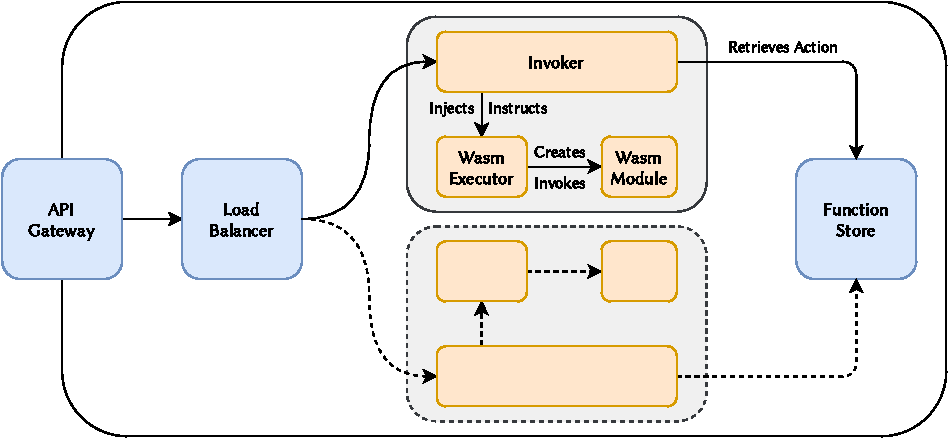
\includegraphics{figures/WasmOpenWhiskActionInvocationFlow.pdf}
    \caption{Invocation flow of a Wasm action in our modified Apache OpenWhisk. The Invoker \emph{injects} the code into the executor which \emph{creates} a Wasm Module ready for execution. It then \emph{instructs} the executor to \emph{invoke} the module with the parameters it passes. The result is passed back to the Invoker. Again, a deployer can define whether one or more Invokers exist.}
    \label{fig:wasm-openwhisk-action-invocation-flow}
\end{figure}

In figure \ref{fig:wasm-openwhisk-action-invocation-flow} we have sketched the high-level modifications that we need to make to OpenWhisk. In this invocation flow, we need to modify OpenWhisk's \inl{Invoker} such that it communicates with the Wasm executor instead of the Docker daemon. Fortunately, the \inl{Invoker} is already well-separated from the concrete containerization technology through a Service Provider Interface (SPI). As previously mentioned, OpenWhisk supports Docker as well as Kubernetes through the \inl{ContainerFactory} trait. We add a \inl{WasmContainerFactory} that implements this trait. Via a property, we can instruct OpenWhisk to use this factory. It uses a \inl{WasmClient}, that can start and destroy a container by invoking the endpoints of the same name on the Wasm executor. The start function returns its result as a \inl{WasmContainer} that extends OpenWhisk's \inl{Container} abstraction. This trait handles container communication, such as calling the \inl{/init} and \inl{/run} endpoints. It also implements \inl{suspend} and \inl{resume} functions, which we do not implement. Docker containers potentially use CPU cycles and memory while they are up, so vanilla OpenWhisk pauses them between invocations, which suspends all of its processes and prevents them from using the CPU. Containers in our executor, on the other hand, consume only memory but no CPU in-between requests, so pausing is not a meaningful operation. The \inl{Container} also allows collecting the logs that an action produced. This is not strictly necessary functionality for correct operation, so we do not implement it. Since we want to implement three runtimes in our executor, keeping the requirements for each of them minimal is important. However, implementing a log mechanism with WASI is entirely possible.

% Figure that shows a zoomed-in version of the invoker and its SPIs (as well as the Wasm executor?) - Help better understand OW's design and what we added

In OpenWhisk's Docker container implementation, OpenWhisk only uses the Docker daemon to create a container, but then communicates with the container directly. In our implementation, every request is proxied through the Wasm executor to the container itself. This design presupposes that the Wasm executor can handle a large amount of concurrent requests, which we noted in our requirements. The advantage is, that not every Wasm module needs to implement the OpenWhisk protocol, as discussed under the \inl{krustlet} topic before. The disadvantage is the single point of failure. However, that is mitigated by the bigger picture of OpenWhisk. In a truly resilient deployment, we would have multiple \inl{Invoker}s. A failing Wasm executor would let the entire \inl{Invoker} unit fail, but other \inl{Invoker}s could take over requests. Furthermore, the executor itself could be scheduled as, e.g. a Kubernetes pod with a restart policy of \inl{Always}. Finally, because WebAssembly runtimes isolate faults of their containers, it is impossible for a faulty Wasm module to affect the entire executor -- barring bugs in the runtimes. The absence of bugs in the executor and the runtimes -- or, at least as small likelihood of their existence -- is therefore also a basic requirement. The mentioned handling of concurrent requests further imply that thread-safety is another one. We noted both of these requirements under the umbrella term of program correctness.
The executor also needs to be generally fast, in order to aid in alleviating the cold start problem. That includes efficient handling of receiving the module's code from OpenWhisk, instantiating it and setting up the underlying Wasm executor. In order to enable execution on all kinds of platforms, including edge devices, another requirement is the executor's ability to run on different instruction set architectures.

\section{Executor implementation}


To implement these requirements in Apache OpenWhisk we will take the following steps. The current Docker-based invoker will be replaced, to forward all the incoming requests to our new Wasm executor.

The Wasm executor will be written from scratch in the Rust\footnote{\url{https://www.rust-lang.org/}} programming language. There are a number of reasons for this choice.

\begin{itemize}
    \item It is a compiled language with performance similar to that of C or C++.
    \item The Rust compiler uses LLVM as its backend so Rust programs can be compiled for any architecture we care about, in particular also \inl{aarch64}. Moreover, we can also compile to \inl{wasm32-wasi}, the WebAssembly WASI target. This allows us to write highly performant WebAssembly modules in Rust, such that we can test our executor \emph{and} the Docker actions under the best possible conditions.
    \item It has good support for asynchronous I/O, so Rust web frameworks can efficiently handle a large amount of concurrent requests.
    \item Program correctness is one of Rust's primary goals, which is enabled through a large amount of guarantees that can be checked at compile time. In particular, writing memory-safe programs is much easier than in C or C++, while providing a similar level of performance.
    \item A subcategory of the preceding point, but worth pointing out: Rust allows for »fearless concurrency«, that is having concurrent programs checked for thread-safety at compile time. In particular, the compiler can detect subtle bugs like data races.
    \item Two of the three used Wasm runtimes are written in Rust, so embedding them is well documented, straightforward and their APIs tend to be the most idiomatic, powerful and up-to-date. The other Wasm runtime, \inl{wamr}, is written in C, which can be efficiently embedded from Rust through bindings.
\end{itemize}

\begin{listing}[ht]
    \begin{minted}{rust}
#[async_std::main]
async fn main() -> anyhow::Result<()> {
    #[cfg(feature = "wasmtime_rt")]
    let runtime = ow_wasmtime::Wasmtime::default();

    #[cfg(feature = "wasmer_rt")]
    let runtime = ow_wasmer::Wasmer::default();

    #[cfg(feature = "wamr_rt")]
    let runtime = ow_wamr::Wamr::default();

    let mut executor = tide::with_state(runtime);

    executor.at("/:container_id/init").post(core::init);
    executor.at("/:container_id/run").post(core::run);
    executor.at("/:container_id/destroy").post(core::destroy);

    executor.listen("127.0.0.1:9000").await.unwrap();

    Ok(())
}
\end{minted}
    \caption{The main function of our WebAssembly executor. The \inl{\#[cfg(feature = "...")]} macros allow us to define multiple runtimes while deciding at compile-time which of them to enable. Thus, we can build three separate binaries, with each only containing the code necessary for its runtime.}
    \label{listing:wasm-executor-main}
\end{listing}

The main function in Listing \ref{listing:wasm-executor-main} suits itself well to describe the high-level architecture of the executor. The entry point into our executor will be through HTTP endpoints. We will not make use of any advanced HTTP features, so the choice of the web framework doesn't matter too much. We use \inl{tide} \cite{Turon2021}, an asynchronous by-default web framework ideal for prototyping. We will discuss asynchronous Rust in greater detail in a later section. Suffice it to say, that the \inl{\#[async\_std::main]} macro starts this program in an asynchronous runtime, which enables us to use \inl{async} functions and \inl{await} them. The async runtime allows multiple concurrent requests to any of the endpoints, without us having to spawn threads explicitly.

We instantiate one of our three implemented Wasm runtimes, only one of which is compiled into the executable, based on the feature flag we pass to the compiler. The runtime is used as \emph{state}, in \inl{tide} terminology, which is to say that it is is injected into each request and thus shared among requests. Sharing objects among threads requires them to be thread-safe. This is where Rust's compile-time checks help us ensure this property. The \inl{tide::with\_state} function can take any argument that implements three traits: \inl{Clone}, \inl{Send} and \inl{Sync}. The first simply gives objects implementing it the ability to be duplicated. This is necessary, such that each request can receive a copy of the runtime. Although, a deep copy would be too expensive for each request. Our runtime wrappers therefore implement \inl{Clone} as a shallow copy, that is, it creates a new reference to the same inner object that all other wrapper objects also point to. For this to work safely, we need the other traits. These are only \emph{marker traits}, indicating that an object satisfies a property. \inl{Send} means a type can be transferred across thread boundaries, while \inl{Sync} means that references to that type can be shared between threads. These properties are satisfied, if the types that we use in the definition of our runtimes and those used transitively, have these properties. That is all to say that the types of the runtimes we use need to be thread-safe, i.e. implement those marker traits. Here is where the differences between the runtimes start to emerge, but we will discuss those in a later section.

To start a container, the \inl{WasmContainer} object in OpenWhisk generates a new universally unique identifier (uuid), without having to communicate with the Wasm executor at all. This is possible because there is no setup for a Wasm container, that needs to happen ahead-of-time, like network namespace creation for Docker containers.
That shows an important aspect of what constitues a WebAssembly container. In-memory, it is ultimately only represented by the action's code. No external operating system resource is used.
It follows, that actual work only happens in the endpoints, which are parameterized by the container id. \inl{/init} is called once by OpenWhisk per container; to initialize the container with the module's code. Although different for each runtime, in general, this endpoint will do any work that can be frontloaded. \inl{/run} is invoked potentially many times, so any work that is not frontloaded would multiply there. Of course, \inl{/init} is the potential culprit for the cold start latency, so our focus is on reducing even the amount of work this endpoint needs to handle. We describe the optimizations towards that end, later in this chapter. Once OpenWhisk decides to destroy the container, it does so through \inl{/destroy}.

% Finally, we give \inl{tide} a function pointer for each endpoint and listen on a local address.

\subsection{Fast cold starts}
In serverless platforms we can identify three important steps, in order for code to be executed. Uploading the code to the platform, initializing the execution environment, and running it. The latter two steps are already part of the execution path; they occurr when an execution request is actively waiting for the result to be returned. Thus, during initialization, the action should already be well-optimized for execution such that as little preparation as possible is needed. WebAssembly is binary target format, however not one, that is ready for \emph{fast} execution. It can be interpreted right away -- thus a small cold start time -- but execution performance will lack behind massively compared to native code, which is unacceptable. So compilation to native code is essential for good runtime performance, but it also takes time for that to be applied to a Wasm module. Given this trade-off, it would seem that Just-in-Time compilation should be the best model. In \inl{wasmtime}, our JIT-runtime of choice, compilation of a simple, WASI-enabled module (1,6 MB) still takes 35 milliseconds on our test machine (or 40 milliseconds when optimizing for speed). This time represents 98\% of the entire setup time, including every other part of the runtime. Thus, unsuprisingly, the cold start is defined almost entirely by the compilation phase. For comparison, the cold start time of the \inl{hello-world} Docker image on the same machine is 452 milliseconds. This number is roughly in line with the cold start times of AWS Lambda or Google Cloud Function, that we've cited in chapter \ref{chapter:background}. While the JIT cold start is an order of magnitude faster than the startup times of Docker containers, it is arguably still on the same order of magnitude as the execution time of some actions. Given that the compilation phase takes up such a big chunk of the overall time, it is the most obvious starting point for further optimizations. And there is room for improvement.

In contrast to browsers, which receive JavaScript or WebAssembly just-in-time, and thus need to compile it in the same manner, a serverless platform takes ownership of a module earlier. When a user uploads a module, the platform has an almost unconstrained amount of time to apply optimizations to the module thereby making it ready for a fast startup \emph{and} execution; solving the previously described dilemma. Thus, the key is to run the expensive module creation ahead of the time of execution. It does not matter in this case, whether the actual execution model of the underlying runtime is JIT or AoT. It's obvious for AoT - the code needs to be compiled ahead of time in its entirety, by definition. As we've seen, JIT also has a cold start penalty and we can complete that step ahead of time, too. We refer to this as precompilation. Once the module is precompiled, we can serialize it and store it in the database. During initialization, all that is left to do is to deserialize precompiled bytes into a \inl{Module} and keep it in memory, which is a very fast operation. At the time of execution, the module is ready to produce an instance and execution can start immediately.

Both \inl{wasmer} and \inl{wamr} support AoT compilation. \inl{wasmer} in particular, allows us to leverage \inl{LLVM} for highly optimized native code to produce a shared object. The runtime loads this via a fast \inl{dlopen} call. \inl{wamr} produces its own AoT format which it can deserialize at runtime and achieve a fast startup as well. For \inl{wasmtime} it is the same in all but the name. We can run the relatively expensive module creation ahead-of-time, and serialize and store the result. Thus, all the runtimes can support some form of precompilation.

\subsection{Warm starts}

Even though the cold start of our executor is well-optimized with this technique, cold starting for every single invocation would still be too expensive for sequential invocations. After all, the \inl{init} procedure still requires retrieving the module from the database and copy it to the executor. We can save on that too, by simply taking advantage of OpenWhisk's current design. In order to adhere to it, we need to store the module between \inl{init} and \inl{run}. The advantage of that is, of course, that after the initialization, \inl{run} can be called again and again, without having to go through any of the setup. This is how OpenWhisk works with Docker containers already. After the initial cold start and first invocation, OpenWhisk pauses the container. If another subsequent request to the same action comes in, it unpauses the container and the action invocation experiences a so-called warm start. This scenario skips the expensive cold start and is much faster. After a threshold without any invocations -- which defaults to 10 minutes -- OpenWhisk calls the \inl{destroy} function on the container, removing it entirely.
Thus, by adhering to OpenWhisk's design, we have support for fast warm starts as well.

The advantage of keeping a module in the executor's memory, is that it is already deserialized and new instances can be instantiated from it immediately. An instance is the runtime's representation of a callable Wasm module. If a module is the equivalent of a Docker image, then the instance is the running Docker container. Note that, unlike Docker-based OpenWhisk, we do not keep instances (containers) in-memory, but only the modules (images). The cost of instantiating an instance is negligible. On our test machine it took, on average, 340 microseconds to setup a \inl{wasmtime} instance and the parts needed for execution. This represents the overhead on every warm invocation. Moreover, two instances can execute concurrently, even if the module itself is not thread-safe, for instance when reentrant execution would be unsafe. Finally, implemented this way, it would also be safe to execute two requests from different users, since instances are isolated from each other. They operate on their own memory space and have their own WASI environment. Thus, caching modules rather than instances is a good trade-off.

One potential inefficiency of our design is that our executor stores every container's module once. If OpenWhisk decides to create two containers \inl{A} and \inl{B}, both containing the same module \inl{M}, then \inl{M} will take up memory twice. One reason for that design is that in OpenWhisk vanilla, containers are completely separated from each other and no such optimization would be possible. Our executor is a more centralized solution and would allow for this optimization in the first place. Currently, we trade memory for speed and store the module per container. Thus, adding or removing a container is a fast insert or remove operation on the HashMap.
% Reasons against this optimization are that it increases complexity, is partially unnecessary and may impact performance.
% One reason against this design, however, is the initialization and eviction process.
Internally, the executor uses a thread-safe HashMap to store the modules and let many tasks or threads work with it simultaneously. A store-modules-once approach would require a global lock on the HashMap. During initialization, the executor needs to check whether the module already exists in the HashMap and if it does, increase its atomic reference count. This is already a critical section, since without synchronization, a concurrent destroy operation may have removed the module between the existence check and the increment. Consequently, this requires a global lock on the HashMap to avoid race conditions. This is probably not a performance issue, since lock contention is unlikely given that the average time between container starts or removals is much longer than the amount of time the lock needs to be held.

% We instead trade memory for speed and store the module per container. Thus, adding and removing a container is a trivial and fast insert or remove operation on the HashMap.
% Outside of such workloads, multiple containers with the same module are less likely to be started.

The strongest point against it, however, is whether it would actually help reduce resource waste.
In practice, the naive implementation is only wasting memory, when containers for the same action are started. This primarily happens under bursty or batch workloads. Outside of such workloads, multiple containers with the same module are less likely to be started. But as we've seen in Chapter \ref{chapter:background}, an analysis of open-source serverless applications showed 84\% of them having bursty workloads \cite{Eismann2021}. The likelihood of receiving concurrent requests for the same action and in turn having to create multiple containers is quite high.
This is less of an issue in light of OpenWhisk's per-action concurrency limit. This limit states how many concurrent invocations a container should handle at most. If we increase this value beyond its default of one, then OpenWhisk will send invocation requests for the same action to the same container, up to that limit, without starting a new container and thus duplicating the module in the executor. In particular, figure \ref{fig:openwhisk-concurrency-limit-greater-one} shows how a module can be reused in the same container -- skipping the initialization entirely. Making use of this limit can thus be very important for performance. With a concurrency limit $c$, appropriate for the underlying hardware and workload, up to $c$ requests could be handled by a single container.
Because of these considerations we decided adding this optimization was not necessary.

\begin{figure}
    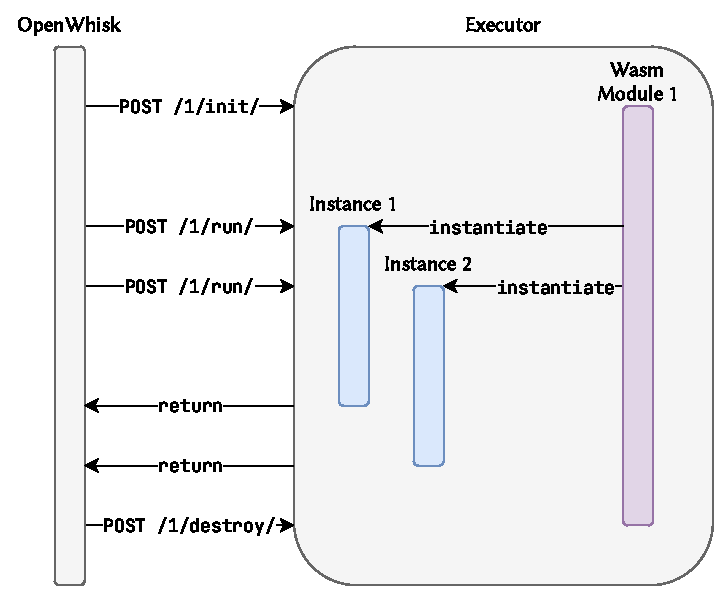
\includegraphics{figures/OpenWhiskConcurrencyLimitGreaterOne.pdf}
    \caption{An example of a container's life cycle when OpenWhisk's concurrency limit is set to a value greater one for that action. Note that a container is only represented in-memory by its module and instances, which is why there is no explicit »container« label in the figure. The container is initialized with a module by OpenWhisk's call to \inl{/init}. Every \inl{/run} request to the same container id spawns a new instance of a WebAssembly module. In particular, two concurrent requests to \inl{/run} can be executed concurrently by the same container. In that case, the instances are instantiated from the same module. The instances are the actual »containers« here, since they are the ones who are isolated from each other and the host. They are short-lived and never reused to guarantee that isolation, i.e. there is a one-to-one relationship between \inl{/run} requests and instances. The Wasm module will stay in memory until OpenWhisk's explicit call to \inl{/destroy}, which occurs after a container has been idle for some threshold time.}
    \label{fig:openwhisk-concurrency-limit-greater-one}
\end{figure}

\subsection{The WasmRuntime abstraction}

\begin{listing}[ht]
    \begin{minted}{rust}
pub trait WasmRuntime: Clone {
    fn initialize(
        &self,
        container_id: String,
        capabilities: ActionCapabilities,
        module: Vec<u8>,
    ) -> anyhow::Result<()>;

    fn run(
        &self,
        container_id: &str,
        parameters: serde_json::Value,
    ) -> Result<Result<serde_json::Value, serde_json::Value>, anyhow::Error>;

    fn destroy(&self, container_id: &str);
}
\end{minted}
    \caption{The \inl{WasmRuntime} abstraction that each of our Wasm runtime wrappers implements. Note the previously mentioned \inl{Clone} trait that is required for using a \inl{WasmRuntime} object as \inl{tide} state. This is required here through the \emph{trait bound}, which means the type implementing this trait needs to also implement \inl{Clone}.}
    \label{listing:wasm-executor-trait}
\end{listing}


The Wasm executor is generic over the underlying WebAssembly runtime, such that we can easily implement different ones and facilitate our comparison. To that end, we abstract the common runtime tasks into a trait -- essentially an interface in Rust's terminology. It is shown in Listing \ref{listing:wasm-executor-trait}. The state of our executor can be any object that implements this trait. For each Wasm runtime we have selected, we implement a wrapper, each of which implements the \inl{WasmRuntime} trait. All our wrapper implementations work in similar ways and differ in details. We describe the implementation for each trait method in the wrappers, while pointing out the important differences between runtimes. Afterwards, we discuss alternatives.

\subsubsection{Initialization}
The executor decodes the base64 string given by OpenWhisk and unzips it, before calling \inl{initialize} with the result. The function initializes the container identified by the given id. All wrappers store the code they're given in a thread-safe HashMap -- provided by the \inl{dashmap}\footnote{\url{https://crates.io/crates/dashmap}} library.

A note on WebAssembly runtime terminology first, based on \inl{wasmtime}'s\footnote{\url{https://docs.rs/wasmtime}} and \inl{wasmer}'s\footnote{\url{https://docs.wasmer.io/integrations/examples/instance}} documentation and the WebAssembly specification\footnote{\url{https://webassembly.github.io/spec/core/exec/runtime.html}}. An engine is used for compiling and managing modules. Recall that a module represents compiled WebAssembly code, similar to a container image, and an instance is the callable instantiation of that code, i.e. the running container. A store is necessary to hold on to memories, tables, functions and other auxiliary data structures.

\begin{description}[style=multiline, leftmargin=2.5cm, font=\bfseries]

    \item[Wasmtime] In \inl{wasmtime}, we instantiate a single, global \inl{Engine} when the executor starts up, which is then used to instantiate all \inl{Module}s. The bytes passed through \inl{initialize} are deserialized into a \inl{Module}, which is a fast operation, and then stored in the internal HashMap. This is possible because a \inl{Module} is thread-safe so the containing HashMap can be safely shared across threads.

    \item[Wasmer] \todo{this} In \inl{wasmer} we store both an \inl{Engine} and a \inl{Store} globally, since a \inl{Module} requires both for instantiation. We will see whether and how that affects memory consumption in chapter \ref{chapter:evaluation}. Like in \inl{wasmtime}, the \inl{Module} is thread-safe.

    \item[Wamr] \inl{wamr} is originally written in C, and we use \inl{wamr\_sys} \footnote{\url{https://crates.io/crates/wamr\_sys}} bindings to embed it in Rust. Contrary to the other runtimes, a module in \inl{wamr} is not thread-safe. Thus, only the serialized bytes representing the module are stored in the HashMap. It follows that the deserialization happens in every \inl{run} call instead, which is slightly more expensive.
    Additionally, two functions need to be called globally for the runtime to be instantiated and torn down, \inl{wasm\_runtime\_init} and \inl{wasm\_runtime\_destroy}, respectively.
    Our implementation requires each runtime state to implement \inl{Clone}. A common pattern in Rust (also used by \inl{wasmtime} and \inl{wasmer}) is to implement the clone operation to produce a shallow copy. Internally, these objects typically use Rust's atomically reference-counted smart pointer (\inl{Arc}) to store a pointer to the actual object, in order to safely share this object across threads. This makes it cheap to share the wrapper object across different threads while having access to the same underlying data. On each request a clone of the runtime is created and destroyed (dropped) at the end. Because of that we cannot call \inl{wasm\_runtime\_destroy} in the wrapper's \inl{Drop} implementation. Instead, we use another internal Arc, which is instantiated with an object that calls the initialization function when it is created, and destroys the context when it is being dropped. Because the \inl{Arc} will live as long as the runtime and only calls the contained object's \inl{drop} function when all other references have gone away, this implements our requirements. This also shows that \inl{wamr}'s API is harder to use safely and correctly, than the idiomatic Rust API's of the other runtimes.

\end{description}

Both \inl{wasmtime} and \inl{wasmer} underline the importance of the validity of the bytes given to the respective \inl{deserialize} methods. Unlike a Wasm module, the compilation artifacts can not be validated in the same way since they already represent a compiled module. So they have to be trusted, when the corresponding Wasm module would not have to be trusted. In our prototype, the users actually supply the compilation artifacts themselves, for development convenience reasons. For an actual serverless framework making use of Wasm, it would have to take ownership of the Wasm module and do the precompilation itself, in order to trust the code.

\subsubsection{Execution}

All runtimes implemented support the WebAssembly System Interface. Recall that WASI follows a capability-based security model, which allows for fine-grained control over what the module has access to. Hence, building a WASI context means setting up those capabilities, like forwarding \inl{stdin} or receiving from \inl{stdout}, setting environment variables or \inl{argv}. By default, the module also has access to WASI APIs like \inl{random\_get} for high-quality randomness or \inl{clock\_time\_get} to attain values from various clocks. WASI also controls on a per file descriptor basis, what directories the module has access to. Specifically, the modules needs a preopened file descriptor in order to access files. The Wasm runtimes therefore open the files and pass them to the module. However, that information is not present in OpenWhisk since Docker doesn't require it, so we need a way for users to specify these capabilities.

OpenWhisk actions can have optional annotations attached to them, which are simple key-value pairs. We can use those to let users specify capabilities. For instance:

\begin{minted}{sh}
wsk action create cache cache.wasm --annotation dir "/tmp/cache"
\end{minted}

Here a new action named \inl{cache} is created from a file \inl{cache.wasm} with the \inl{wsk} cli tool. A key-value pair is attached with \inl{dir=/tmp/cache}. With some minimal code changes to OpenWhisk's container abstraction, these annotations are then passed to the executor during \inl{initialize}. On the executor side, it is passed to each runtime which can then act on that information. It would be easily possible for a service provider to implement policies on top of it. Access could only be granted to the \inl{/tmp} directory in general; or a default cache directory \inl{/tmp/<container\_id>} could be created for each container, where information can be cached but only \emph{that} container has access to it. As WASI is currently under heavy development and doesn't, for example, specify any network-related interfaces, the amount of capabilities is limited. Our prototype implements directory access and our self-provided HTTP GET request. The latter is relevant to implement a network I/O-bound function for our evaluation in chapter \ref{chapter:evaluation}.


\begin{listing}[ht]
    \begin{minted}{rust}
ow_wasm_action::pass_json!(handler);

pub fn handler(json: serde_json::Value) -> Result<serde_json::Value, anyhow::Error> {
    let param1 = json
        .get("param1")
        .ok_or_else(|| anyhow::anyhow!("Expected param1 to be present"))?
        .as_i64()
        .ok_or_else(|| anyhow::anyhow!("Expected param1 to be an i64"))?;

    let param2 = json
        .get("param2")
        .ok_or_else(|| anyhow::anyhow!("Expected param2 to be present"))?
        .as_i64()
        .ok_or_else(|| anyhow::anyhow!("Expected param2 to be an i64"))?;

    Ok(serde_json::json!({ "result": param1 + param2 }))
}
\end{minted}
    \caption{A simple add action in Rust that uses a macro from \inl{ow-wasm-action} to pass the received json to the \inl{handler} and return the \inl{Result} back to the runtime.}
    \label{listing:add-action-example}
\end{listing}

\inl{run} executes the module associated with the given container id and with the given parameters as input. As required by OpenWhisk, the parameter is a JSON object. The WebAssembly minimum-viable product (MVP), only supports integer data types natively. Higher-level data types often differ in their implementation details between languages, so a universal target format like Wasm cannot decide for one of them, without shutting certain languages out or making it harder for them to be used. Making Wasm modules compiled from different source languages interoperable is an ongoing process -- with WebAssembly interface types\footnote{\url{https://hacks.mozilla.org/2019/08/webassembly-interface-types/}}. The \inl{wasm-bindgen} Rust library already makes this process easy for JavaScript-WebAssembly interoperability. Unfortunately, it does not work with any of our runtimes. Even if both our runtime and the module is written in Rust originally, passing a pointer is not possible because WebAssembly is sandboxed and could not access the pointee. To pass a complex type like a JSON object to the module, we require that it uses a wrapper. Internally, the wrapper allocates a global buffer of bytes. It exports three functions to work with this buffer, most notably one that returns a pointer. When executing the module, the runtime serializes the JSON object as bytes and allocates enough space in the buffer to store them. It then acquires the pointer, which is relative to the module's memory's base pointer, offsets it appropriately and writes the JSON bytes into the buffer. Since the module doesn't know the number of bytes written, the runtime passes that as its argument. On the other side, the module reads the given number of bytes from the buffer and calls the user-provided handler function. Reading the return value of the action uses the same process. Conveniently, the user only has to implement a function that takes a JSON object and returns one in the success case; an error otherwise. Thus, this crude method of passing parameters can be completely hidden from action developers. A simple action can be seen in listing \ref{listing:add-action-example}. The action development process is visualized in figure \ref{fig:action-creation-flow}, which makes use of the \inl{binaryen}\footnote{\url{https://github.com/WebAssembly/binaryen}} toolchain to optimize the Rust-produced WebAssembly.
The mentioned \inl{ow-wasmtime-precompiler} is a crude wrapper around \inl{wasmtime}'s API that creates a module from Wasm bytes, which kicks off the internal compilation process. Once the module is created, it is ready for execution. At this point, we serialize it to a file and zip it. This process compiles the module for the current host architecture. \inl{wamrc} and \inl{wasmer compile} can also take a target argument to precompile for a different host, e.g. a Raspberry Pi with the \inl{aarch64} ISA. However, as of version \inl{0.26}, the \inl{wasmtime} cli has also gained similar capabilities.
% One point of interest is the memory allcator. Because Wasm's original use case is in the web browser, where the binary is downloaded just-in-time, the binary size matters. Thus, a smaller memory allocator was written for Rust, named \inl{wee_alloc}\footnote{\url{https://github.com/rustwasm/wee_alloc}}. It effectively trades performance for a smaller size. Since we precompile our WebAssembly the size difference is negligible. If we were not precompiling, this might be a more interesting feature to activate.

\begin{figure}
    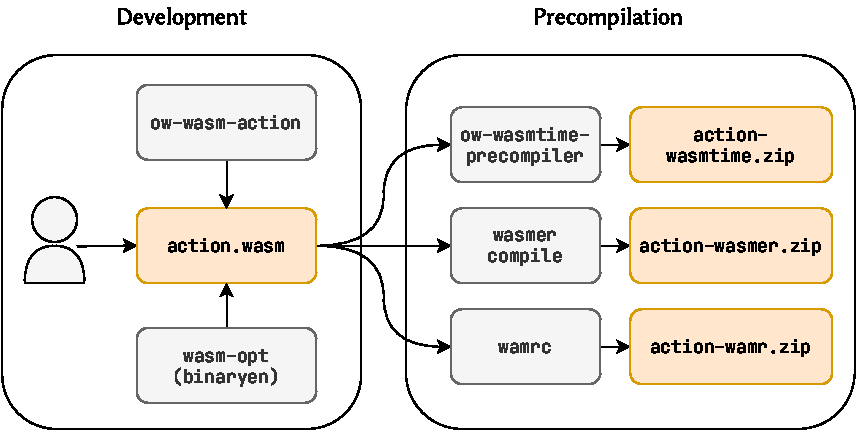
\includegraphics{figures/ActionCreationFlow.pdf}
    \caption{There are two phases in the action development. Our \inl{ow-wasm-action} library provides the abstraction to read the parameters the runtime has passed and to write the return value. To that end, it uses \inl{serde\_json}, a (de)serialization library to read and write the JSON objects. Afterwards, \inl{wasm-opt} runs an optimization pass on the produced WebAssembly, since not all runtimes run an extensive optimization pass.
    Depending on what runtime is compiled into the executor, the corresponding precompiler needs to be used. For \inl{wasmtime}, we have written the small \inl{ow-wasmtime-precompiler} program that precompiles the Wasm code into a format ready for execution, while \inl{wamrc} and \inl{wasmer compile} can be used for the others. Finally, the resulting precompiled binary is zipped which reduces the transmission size and instructs OpenWhisk cli to treat it as binary. The zip file is then ready to be uploaded to OpenWhisk.}
    \label{fig:action-creation-flow}
\end{figure}

The creation of the WASI context as well as the actual execution is slightly different for each runtime.

% The \inl{Store} is only needed to instantiate an \inl{Instance}, and should not be long-lived, according to the documentation. Thus, these two data structures are instantiated per-request, in each \inl{/run} invocation, and discarded afterwards. Evidently, this runtime's API is a very good fit for our use case.

\begin{description}[style=multiline, leftmargin=2.5cm, font=\bfseries]

    \item[Wasmtime] The \inl{wasmtime} runtime, as of version \inl{0.23}, uses \inl{cap-std}, a capability based implementation with a similar API as the Rust standard libary. We can construct its \inl{Dir} type and use it while building a \inl{WasiCtxBuilder}, ultimately yielding a \inl{WasiCtx}. The context is \emph{linked} with the module using the runtime's \inl{Linker}, which is similar to an operating system's dynamic linker. It resolves the imports that the module needs and instantiates it with them.
          To execute, we create a \inl{Store} per request, thus per \inl{run} invocation. This is because a \inl{Store} is neither thread-safe nor meant to be long-lived, according to the documentation. The \inl{Store} is used as a collection of the instances and the host-defined items, according to the documentation.

    \item[Wasmer] In \inl{wasmer} we build up a \inl{WasiEnv} with a very similar API as \inl{wasmtime}'s, including directory access. The module and environment are combined into an \inl{ImportObject} from which an \inl{Instance} is instantiated.

    \item[Wamr] \inl{wamr}'s API is slightly lower-level and less ergonomic compared to the other runtimes due to it being a C-API rather than an idiomatic Rust one.
    

\end{description}

So in summary -- across all runtimes -- \inl{run} looks up the previously stored module with the container id, creates a WASI context with the associated capabilities, passes the parameters and executes the module's default function. If an error occurs during the Wasm runtime setup, the outer \inl{Result} contains an \inl{anyhow::Error}, a generic, application-level error type. Since the Wasm module itself can also either succeed or fail, another \inl{Result} is nested inside, where both success and failure are represented by JSON objects.

In what task or thread the module is executed, will be discussed shortly.

\subsubsection{Cleanup}
Finally, the \inl{destroy} function removes the container, which simply means freeing the memory taken up by the module. This is fast and thread-safe, since each container manages its own Wasm module. Once OpenWhisk has decided to destroy the container, it will synchronize internally to not call \inl{run} on it again.

An overview of the entire executor workflow can be seen in figure \ref{fig:executor-overview}.

\begin{figure}
    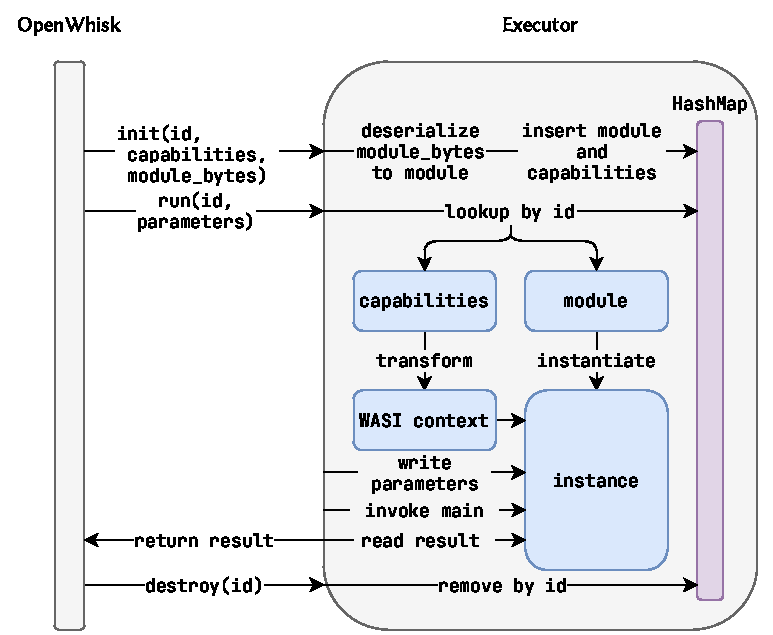
\includegraphics{figures/ExecutorOverview.pdf}
    \caption{An overview of the executor architecture. \inl{init} decodes the received bytes using \inl{base64} and unzips the result. From there they are deserialized back into a \inl{Module} instance, in the case of \inl{wasmtime} and \inl{wasmer}. The module and capabilities are then stored in the HashMap. When a \inl{run} request comes in, the module and capabilities are looked up. The capabilities are transformed to a WASI context (named differently under different runtimes), which is used to instantiate an instance, together with the module. The parameters for this \inl{run} request are serialized to JSON and written into the instance's memory. When its \inl{main()} function is invoked, the JSON is deserialized and passed to the actual handler function. The result is returned to OpenWhisk. A \inl{destroy} request simply translates to a remove operation on the HashMap. Note that this figure is accurate for \inl{wasmtime} and \inl{wasmer}, but not entirely for \inl{wamr}. The latter runtime's module creation is slightly different, as explained above.}
    \label{fig:executor-overview}
\end{figure}

\subsection{Implementation alternatives}
Instead of caching modules some may wish to cache instances instead. The case for reusing instances is to avoid costly setup in the action itself, like connection pools to external resources or to avoid rebuilding a cache on every request.
We need to manage instances in that case, i.e. we need a pool of instances and a management system around it. When a new request comes in, we would ideally like to reuse an existing instance. That requires synchronizing with other threads, to decide which thread gets to reuse an instance and which needs to create a new one. We would need per-instance synchronization to check whether an instance is currently in use or usable. It is questionable whether the synchronization overhead would be less costly than always creating a new instance, in particular because creating instances is a relatively cheap operation. For this reason we decided against it.

% As seen in figure \ref{fig:executor-overview}, a WASI context is created per \inl{run} invocation. If a module needs access to a file for instance, creating the context requires requires opening file descriptors. Similarly, with a future network API in WASI, this might require invoking more system calls. These calls may not be expensive per-se, but as we've seen in this work as a whole, frontloading resource instantiation as much as possible can have net performance benefits. In particular, if it's possible to pre-create the WASI context we should do it. In \inl{wasmtime} this is not possible, because the \inl{WasiCtx} is not thread-safe. In \inl{wasmer} on other hand, the \inl{WasiEnv} is thread-safe and can be cheaply cloned to send across threads. With both runtimes, we are creating one context per instance.

% Furthermore, with a new instance per request, we have per request isolation and fully stateless execution -- something that the action developer can rely upon.



\subsection{Enabling concurrency}

In order for our executor to handle requests to these endpoints concurrently, we use Rust's \inl{async} features. It is a programming model that »lets you run a large number of concurrent tasks on a small number of OS threads« \cite{AsyncBook2021}. With this model a high number of I/O-bound tasks can be handled with less resources than a thread-based model could. The question then becomes, whether executing WebAssembly modules is I/O-bound. The answer, of course, is that it depends on the WebAssembly module! If the module calculates a large prime number, the task is CPU-bound; but if it reads a file from disk and returns it, it is I/O-bound.
Whether serverless workloads are primarily one or the other is not well researched. However, we can make an educated guess. As we have seen in chapter \ref{chapter:background}, the majority of serverless functions are written in JavaScript in the \inl{node.js} engine or in Python... 

The executor consists of a web server that can take requests from the invoker asynchronously and concurrently. Because OpenWhisk doesn't communicate with the Wasm modules directly, but through the executor, the \inl{/start} endpoint simply returns the executors own network address. This endpoint also returns an identifier for the container, so that OpenWhisk can handle its life cycle, i.e. the above-mentioned mechanism of keeping it warm for some time, for a faster subsequent invocation. There is a chance that this mechanism may not be necessary for Wasm modules, as they are much more lightweight in their instantiation. We will come back to this question later in our optimization discussion.


Rust's async model works with \inl{Futures} -- also known as Promises in JavaScript -- which represent values that have not yet been computed. Contrary to \inl{Promises} however, Rust's \inl{Futures} are lazy: They do nothing unless actively polled. This task falls to \inl{async} runtimes, of which \inl{async-std} provides one. In \inl{async-std} the unit of execution is a \inl{Task}, which is similar to a \inl{Thread}, except it is driven to completion by the user space runtime instead of the OS. Many of those tasks are executed on the same thread, and by default, a \inl{Thread} per logical CPU core is spawned. Thus we have $M \cdot N$ tasks in total, where $M$ is the number of tasks per thread and $N$ the number of logical CPU cores.
From that, a second distinction is implied. A \inl{Task} should not do a blocking or long-running operation, like reading from a file via the standard library's \inl{std::fs::read\_to\_string}. Instead, it should use the \inl{async} version of that method, from \inl{async-std}, which does not block the thread. Otherwise, all other $M - 1$ tasks, which are executed on the same thread, will also be blocked, even though they may be able to make progress. Note that, we could still process $N$ requests concurrently, even if tasks block, but that doesn't scale well enough. This is why these kinds of async functions are also called cooperative routines (coroutines). When they need to wait for the OS to finish a task, they \emph{yield} to another routine, which can then continue actual work.

That becomes relevant for us, when we execute WebAssembly modules. Taking the module, setting up the Wasm runtime and executing it, is a long-running computation -- and one that could block as well. This would in turn block the thread we are currently running on, which means, only $N$ Wasm modules can be executed concurrently. This is not an issue for computationally-intensive workloads, where no more work can be done concurrently, than the CPU has logical cores. However, for I/O-bound workloads, such as requests over the network, this can quickly become a bottleneck. Since one of the appealing offerings of serverless frameworks is their elasticity, we clearly need a way to handle many more requests, even if they block.
To let other coroutines on the same thread make progress, while one executes the module, we can push the entire execution onto a thread pool. The coroutine then has the simple job to asynchronously wait for that execution to finish and collect the result. That allows the other coroutines to process more requests in the meantime.

To test the theory, whether the thread pool model is able to handle more requests, we run two short experiments.

\begin{enumerate}
    \item Compute-bound: Calculating a large prime number.
          % \item Filesystem-I/O-bound: Reading a 30 MB file from disk.
    \item Network-I/O-bound: Making a long-running (1 second) HTTP request.
\end{enumerate}

Our test machine has 8 logical CPU cores, resulting in 8 threads being started for the async-std runtime. We thus send 16 concurrent requests to be able to see the potential blocking in the result. The first experiment showed no difference in the total execution time between the default and thread pool model. As we would expect, in the default model the compute-bound task finishes the first 8 requests, before starting the second set. The execution in a thread pool executes all 16 requests concurrently, but each took roughly twice as long, resulting in no significant difference between the total execution time. The default model operates more along the first-come, first-serve principle, where an early request will also get a response more quickly. In this simplified example, where all workloads are compute-bound, this may be preferable.

\begin{figure}
    \begin{center}
        %% Creator: Matplotlib, PGF backend
%%
%% To include the figure in your LaTeX document, write
%%   \input{<filename>.pgf}
%%
%% Make sure the required packages are loaded in your preamble
%%   \usepackage{pgf}
%%
%% and, on pdftex
%%   \usepackage[utf8]{inputenc}\DeclareUnicodeCharacter{2212}{-}
%%
%% or, on luatex and xetex
%%   \usepackage{unicode-math}
%%
%% Figures using additional raster images can only be included by \input if
%% they are in the same directory as the main LaTeX file. For loading figures
%% from other directories you can use the `import` package
%%   \usepackage{import}
%%
%% and then include the figures with
%%   \import{<path to file>}{<filename>.pgf}
%%
%% Matplotlib used the following preamble
%%   \usepackage{fontspec}
%%
\begingroup%
\makeatletter%
\begin{pgfpicture}%
\pgfpathrectangle{\pgfpointorigin}{\pgfqpoint{5.809079in}{4.647263in}}%
\pgfusepath{use as bounding box, clip}%
\begin{pgfscope}%
\pgfsetbuttcap%
\pgfsetmiterjoin%
\definecolor{currentfill}{rgb}{1.000000,1.000000,1.000000}%
\pgfsetfillcolor{currentfill}%
\pgfsetlinewidth{0.000000pt}%
\definecolor{currentstroke}{rgb}{1.000000,1.000000,1.000000}%
\pgfsetstrokecolor{currentstroke}%
\pgfsetdash{}{0pt}%
\pgfpathmoveto{\pgfqpoint{0.000000in}{0.000000in}}%
\pgfpathlineto{\pgfqpoint{5.809079in}{0.000000in}}%
\pgfpathlineto{\pgfqpoint{5.809079in}{4.647263in}}%
\pgfpathlineto{\pgfqpoint{0.000000in}{4.647263in}}%
\pgfpathclose%
\pgfusepath{fill}%
\end{pgfscope}%
\begin{pgfscope}%
\pgfsetbuttcap%
\pgfsetmiterjoin%
\definecolor{currentfill}{rgb}{0.917647,0.917647,0.949020}%
\pgfsetfillcolor{currentfill}%
\pgfsetlinewidth{0.000000pt}%
\definecolor{currentstroke}{rgb}{0.000000,0.000000,0.000000}%
\pgfsetstrokecolor{currentstroke}%
\pgfsetstrokeopacity{0.000000}%
\pgfsetdash{}{0pt}%
\pgfpathmoveto{\pgfqpoint{0.667583in}{2.791604in}}%
\pgfpathlineto{\pgfqpoint{5.629079in}{2.791604in}}%
\pgfpathlineto{\pgfqpoint{5.629079in}{4.266596in}}%
\pgfpathlineto{\pgfqpoint{0.667583in}{4.266596in}}%
\pgfpathclose%
\pgfusepath{fill}%
\end{pgfscope}%
\begin{pgfscope}%
\pgfpathrectangle{\pgfqpoint{0.667583in}{2.791604in}}{\pgfqpoint{4.961496in}{1.474993in}}%
\pgfusepath{clip}%
\pgfsetroundcap%
\pgfsetroundjoin%
\pgfsetlinewidth{1.003750pt}%
\definecolor{currentstroke}{rgb}{1.000000,1.000000,1.000000}%
\pgfsetstrokecolor{currentstroke}%
\pgfsetdash{}{0pt}%
\pgfpathmoveto{\pgfqpoint{0.893106in}{2.791604in}}%
\pgfpathlineto{\pgfqpoint{0.893106in}{4.266596in}}%
\pgfusepath{stroke}%
\end{pgfscope}%
\begin{pgfscope}%
\definecolor{textcolor}{rgb}{0.150000,0.150000,0.150000}%
\pgfsetstrokecolor{textcolor}%
\pgfsetfillcolor{textcolor}%
\pgftext[x=0.893106in,y=2.659659in,,top]{\color{textcolor}\rmfamily\fontsize{11.000000}{13.200000}\selectfont \(\displaystyle {0.00}\)}%
\end{pgfscope}%
\begin{pgfscope}%
\pgfpathrectangle{\pgfqpoint{0.667583in}{2.791604in}}{\pgfqpoint{4.961496in}{1.474993in}}%
\pgfusepath{clip}%
\pgfsetroundcap%
\pgfsetroundjoin%
\pgfsetlinewidth{1.003750pt}%
\definecolor{currentstroke}{rgb}{1.000000,1.000000,1.000000}%
\pgfsetstrokecolor{currentstroke}%
\pgfsetdash{}{0pt}%
\pgfpathmoveto{\pgfqpoint{1.456912in}{2.791604in}}%
\pgfpathlineto{\pgfqpoint{1.456912in}{4.266596in}}%
\pgfusepath{stroke}%
\end{pgfscope}%
\begin{pgfscope}%
\definecolor{textcolor}{rgb}{0.150000,0.150000,0.150000}%
\pgfsetstrokecolor{textcolor}%
\pgfsetfillcolor{textcolor}%
\pgftext[x=1.456912in,y=2.659659in,,top]{\color{textcolor}\rmfamily\fontsize{11.000000}{13.200000}\selectfont \(\displaystyle {0.25}\)}%
\end{pgfscope}%
\begin{pgfscope}%
\pgfpathrectangle{\pgfqpoint{0.667583in}{2.791604in}}{\pgfqpoint{4.961496in}{1.474993in}}%
\pgfusepath{clip}%
\pgfsetroundcap%
\pgfsetroundjoin%
\pgfsetlinewidth{1.003750pt}%
\definecolor{currentstroke}{rgb}{1.000000,1.000000,1.000000}%
\pgfsetstrokecolor{currentstroke}%
\pgfsetdash{}{0pt}%
\pgfpathmoveto{\pgfqpoint{2.020718in}{2.791604in}}%
\pgfpathlineto{\pgfqpoint{2.020718in}{4.266596in}}%
\pgfusepath{stroke}%
\end{pgfscope}%
\begin{pgfscope}%
\definecolor{textcolor}{rgb}{0.150000,0.150000,0.150000}%
\pgfsetstrokecolor{textcolor}%
\pgfsetfillcolor{textcolor}%
\pgftext[x=2.020718in,y=2.659659in,,top]{\color{textcolor}\rmfamily\fontsize{11.000000}{13.200000}\selectfont \(\displaystyle {0.50}\)}%
\end{pgfscope}%
\begin{pgfscope}%
\pgfpathrectangle{\pgfqpoint{0.667583in}{2.791604in}}{\pgfqpoint{4.961496in}{1.474993in}}%
\pgfusepath{clip}%
\pgfsetroundcap%
\pgfsetroundjoin%
\pgfsetlinewidth{1.003750pt}%
\definecolor{currentstroke}{rgb}{1.000000,1.000000,1.000000}%
\pgfsetstrokecolor{currentstroke}%
\pgfsetdash{}{0pt}%
\pgfpathmoveto{\pgfqpoint{2.584525in}{2.791604in}}%
\pgfpathlineto{\pgfqpoint{2.584525in}{4.266596in}}%
\pgfusepath{stroke}%
\end{pgfscope}%
\begin{pgfscope}%
\definecolor{textcolor}{rgb}{0.150000,0.150000,0.150000}%
\pgfsetstrokecolor{textcolor}%
\pgfsetfillcolor{textcolor}%
\pgftext[x=2.584525in,y=2.659659in,,top]{\color{textcolor}\rmfamily\fontsize{11.000000}{13.200000}\selectfont \(\displaystyle {0.75}\)}%
\end{pgfscope}%
\begin{pgfscope}%
\pgfpathrectangle{\pgfqpoint{0.667583in}{2.791604in}}{\pgfqpoint{4.961496in}{1.474993in}}%
\pgfusepath{clip}%
\pgfsetroundcap%
\pgfsetroundjoin%
\pgfsetlinewidth{1.003750pt}%
\definecolor{currentstroke}{rgb}{1.000000,1.000000,1.000000}%
\pgfsetstrokecolor{currentstroke}%
\pgfsetdash{}{0pt}%
\pgfpathmoveto{\pgfqpoint{3.148331in}{2.791604in}}%
\pgfpathlineto{\pgfqpoint{3.148331in}{4.266596in}}%
\pgfusepath{stroke}%
\end{pgfscope}%
\begin{pgfscope}%
\definecolor{textcolor}{rgb}{0.150000,0.150000,0.150000}%
\pgfsetstrokecolor{textcolor}%
\pgfsetfillcolor{textcolor}%
\pgftext[x=3.148331in,y=2.659659in,,top]{\color{textcolor}\rmfamily\fontsize{11.000000}{13.200000}\selectfont \(\displaystyle {1.00}\)}%
\end{pgfscope}%
\begin{pgfscope}%
\pgfpathrectangle{\pgfqpoint{0.667583in}{2.791604in}}{\pgfqpoint{4.961496in}{1.474993in}}%
\pgfusepath{clip}%
\pgfsetroundcap%
\pgfsetroundjoin%
\pgfsetlinewidth{1.003750pt}%
\definecolor{currentstroke}{rgb}{1.000000,1.000000,1.000000}%
\pgfsetstrokecolor{currentstroke}%
\pgfsetdash{}{0pt}%
\pgfpathmoveto{\pgfqpoint{3.712137in}{2.791604in}}%
\pgfpathlineto{\pgfqpoint{3.712137in}{4.266596in}}%
\pgfusepath{stroke}%
\end{pgfscope}%
\begin{pgfscope}%
\definecolor{textcolor}{rgb}{0.150000,0.150000,0.150000}%
\pgfsetstrokecolor{textcolor}%
\pgfsetfillcolor{textcolor}%
\pgftext[x=3.712137in,y=2.659659in,,top]{\color{textcolor}\rmfamily\fontsize{11.000000}{13.200000}\selectfont \(\displaystyle {1.25}\)}%
\end{pgfscope}%
\begin{pgfscope}%
\pgfpathrectangle{\pgfqpoint{0.667583in}{2.791604in}}{\pgfqpoint{4.961496in}{1.474993in}}%
\pgfusepath{clip}%
\pgfsetroundcap%
\pgfsetroundjoin%
\pgfsetlinewidth{1.003750pt}%
\definecolor{currentstroke}{rgb}{1.000000,1.000000,1.000000}%
\pgfsetstrokecolor{currentstroke}%
\pgfsetdash{}{0pt}%
\pgfpathmoveto{\pgfqpoint{4.275944in}{2.791604in}}%
\pgfpathlineto{\pgfqpoint{4.275944in}{4.266596in}}%
\pgfusepath{stroke}%
\end{pgfscope}%
\begin{pgfscope}%
\definecolor{textcolor}{rgb}{0.150000,0.150000,0.150000}%
\pgfsetstrokecolor{textcolor}%
\pgfsetfillcolor{textcolor}%
\pgftext[x=4.275944in,y=2.659659in,,top]{\color{textcolor}\rmfamily\fontsize{11.000000}{13.200000}\selectfont \(\displaystyle {1.50}\)}%
\end{pgfscope}%
\begin{pgfscope}%
\pgfpathrectangle{\pgfqpoint{0.667583in}{2.791604in}}{\pgfqpoint{4.961496in}{1.474993in}}%
\pgfusepath{clip}%
\pgfsetroundcap%
\pgfsetroundjoin%
\pgfsetlinewidth{1.003750pt}%
\definecolor{currentstroke}{rgb}{1.000000,1.000000,1.000000}%
\pgfsetstrokecolor{currentstroke}%
\pgfsetdash{}{0pt}%
\pgfpathmoveto{\pgfqpoint{4.839750in}{2.791604in}}%
\pgfpathlineto{\pgfqpoint{4.839750in}{4.266596in}}%
\pgfusepath{stroke}%
\end{pgfscope}%
\begin{pgfscope}%
\definecolor{textcolor}{rgb}{0.150000,0.150000,0.150000}%
\pgfsetstrokecolor{textcolor}%
\pgfsetfillcolor{textcolor}%
\pgftext[x=4.839750in,y=2.659659in,,top]{\color{textcolor}\rmfamily\fontsize{11.000000}{13.200000}\selectfont \(\displaystyle {1.75}\)}%
\end{pgfscope}%
\begin{pgfscope}%
\pgfpathrectangle{\pgfqpoint{0.667583in}{2.791604in}}{\pgfqpoint{4.961496in}{1.474993in}}%
\pgfusepath{clip}%
\pgfsetroundcap%
\pgfsetroundjoin%
\pgfsetlinewidth{1.003750pt}%
\definecolor{currentstroke}{rgb}{1.000000,1.000000,1.000000}%
\pgfsetstrokecolor{currentstroke}%
\pgfsetdash{}{0pt}%
\pgfpathmoveto{\pgfqpoint{5.403556in}{2.791604in}}%
\pgfpathlineto{\pgfqpoint{5.403556in}{4.266596in}}%
\pgfusepath{stroke}%
\end{pgfscope}%
\begin{pgfscope}%
\definecolor{textcolor}{rgb}{0.150000,0.150000,0.150000}%
\pgfsetstrokecolor{textcolor}%
\pgfsetfillcolor{textcolor}%
\pgftext[x=5.403556in,y=2.659659in,,top]{\color{textcolor}\rmfamily\fontsize{11.000000}{13.200000}\selectfont \(\displaystyle {2.00}\)}%
\end{pgfscope}%
\begin{pgfscope}%
\pgfpathrectangle{\pgfqpoint{0.667583in}{2.791604in}}{\pgfqpoint{4.961496in}{1.474993in}}%
\pgfusepath{clip}%
\pgfsetroundcap%
\pgfsetroundjoin%
\pgfsetlinewidth{1.003750pt}%
\definecolor{currentstroke}{rgb}{1.000000,1.000000,1.000000}%
\pgfsetstrokecolor{currentstroke}%
\pgfsetdash{}{0pt}%
\pgfpathmoveto{\pgfqpoint{0.667583in}{4.266596in}}%
\pgfpathlineto{\pgfqpoint{5.629079in}{4.266596in}}%
\pgfusepath{stroke}%
\end{pgfscope}%
\begin{pgfscope}%
\definecolor{textcolor}{rgb}{0.150000,0.150000,0.150000}%
\pgfsetstrokecolor{textcolor}%
\pgfsetfillcolor{textcolor}%
\pgftext[x=0.459597in, y=4.213583in, left, base]{\color{textcolor}\rmfamily\fontsize{11.000000}{13.200000}\selectfont \(\displaystyle {0}\)}%
\end{pgfscope}%
\begin{pgfscope}%
\pgfpathrectangle{\pgfqpoint{0.667583in}{2.791604in}}{\pgfqpoint{4.961496in}{1.474993in}}%
\pgfusepath{clip}%
\pgfsetroundcap%
\pgfsetroundjoin%
\pgfsetlinewidth{1.003750pt}%
\definecolor{currentstroke}{rgb}{1.000000,1.000000,1.000000}%
\pgfsetstrokecolor{currentstroke}%
\pgfsetdash{}{0pt}%
\pgfpathmoveto{\pgfqpoint{0.667583in}{3.805661in}}%
\pgfpathlineto{\pgfqpoint{5.629079in}{3.805661in}}%
\pgfusepath{stroke}%
\end{pgfscope}%
\begin{pgfscope}%
\definecolor{textcolor}{rgb}{0.150000,0.150000,0.150000}%
\pgfsetstrokecolor{textcolor}%
\pgfsetfillcolor{textcolor}%
\pgftext[x=0.459597in, y=3.752647in, left, base]{\color{textcolor}\rmfamily\fontsize{11.000000}{13.200000}\selectfont \(\displaystyle {5}\)}%
\end{pgfscope}%
\begin{pgfscope}%
\pgfpathrectangle{\pgfqpoint{0.667583in}{2.791604in}}{\pgfqpoint{4.961496in}{1.474993in}}%
\pgfusepath{clip}%
\pgfsetroundcap%
\pgfsetroundjoin%
\pgfsetlinewidth{1.003750pt}%
\definecolor{currentstroke}{rgb}{1.000000,1.000000,1.000000}%
\pgfsetstrokecolor{currentstroke}%
\pgfsetdash{}{0pt}%
\pgfpathmoveto{\pgfqpoint{0.667583in}{3.344726in}}%
\pgfpathlineto{\pgfqpoint{5.629079in}{3.344726in}}%
\pgfusepath{stroke}%
\end{pgfscope}%
\begin{pgfscope}%
\definecolor{textcolor}{rgb}{0.150000,0.150000,0.150000}%
\pgfsetstrokecolor{textcolor}%
\pgfsetfillcolor{textcolor}%
\pgftext[x=0.383555in, y=3.291712in, left, base]{\color{textcolor}\rmfamily\fontsize{11.000000}{13.200000}\selectfont \(\displaystyle {10}\)}%
\end{pgfscope}%
\begin{pgfscope}%
\pgfpathrectangle{\pgfqpoint{0.667583in}{2.791604in}}{\pgfqpoint{4.961496in}{1.474993in}}%
\pgfusepath{clip}%
\pgfsetroundcap%
\pgfsetroundjoin%
\pgfsetlinewidth{1.003750pt}%
\definecolor{currentstroke}{rgb}{1.000000,1.000000,1.000000}%
\pgfsetstrokecolor{currentstroke}%
\pgfsetdash{}{0pt}%
\pgfpathmoveto{\pgfqpoint{0.667583in}{2.883791in}}%
\pgfpathlineto{\pgfqpoint{5.629079in}{2.883791in}}%
\pgfusepath{stroke}%
\end{pgfscope}%
\begin{pgfscope}%
\definecolor{textcolor}{rgb}{0.150000,0.150000,0.150000}%
\pgfsetstrokecolor{textcolor}%
\pgfsetfillcolor{textcolor}%
\pgftext[x=0.383555in, y=2.830777in, left, base]{\color{textcolor}\rmfamily\fontsize{11.000000}{13.200000}\selectfont \(\displaystyle {15}\)}%
\end{pgfscope}%
\begin{pgfscope}%
\definecolor{textcolor}{rgb}{0.150000,0.150000,0.150000}%
\pgfsetstrokecolor{textcolor}%
\pgfsetfillcolor{textcolor}%
\pgftext[x=0.328000in,y=3.529100in,,bottom,rotate=90.000000]{\color{textcolor}\rmfamily\fontsize{12.000000}{14.400000}\selectfont request number}%
\end{pgfscope}%
\begin{pgfscope}%
\pgfpathrectangle{\pgfqpoint{0.667583in}{2.791604in}}{\pgfqpoint{4.961496in}{1.474993in}}%
\pgfusepath{clip}%
\pgfsetbuttcap%
\pgfsetroundjoin%
\definecolor{currentfill}{rgb}{0.298039,0.447059,0.690196}%
\pgfsetfillcolor{currentfill}%
\pgfsetlinewidth{1.003750pt}%
\definecolor{currentstroke}{rgb}{1.000000,1.000000,1.000000}%
\pgfsetstrokecolor{currentstroke}%
\pgfsetdash{}{0pt}%
\pgfsys@defobject{currentmarker}{\pgfqpoint{0.893106in}{4.197456in}}{\pgfqpoint{3.204001in}{4.243550in}}{%
\pgfpathmoveto{\pgfqpoint{0.893106in}{4.243550in}}%
\pgfpathlineto{\pgfqpoint{0.893106in}{4.197456in}}%
\pgfpathlineto{\pgfqpoint{3.204001in}{4.197456in}}%
\pgfpathlineto{\pgfqpoint{3.204001in}{4.243550in}}%
\pgfpathlineto{\pgfqpoint{0.893106in}{4.243550in}}%
\pgfpathclose%
\pgfusepath{stroke,fill}%
}%
\begin{pgfscope}%
\pgfsys@transformshift{0.000000in}{0.000000in}%
\pgfsys@useobject{currentmarker}{}%
\end{pgfscope}%
\end{pgfscope}%
\begin{pgfscope}%
\pgfpathrectangle{\pgfqpoint{0.667583in}{2.791604in}}{\pgfqpoint{4.961496in}{1.474993in}}%
\pgfusepath{clip}%
\pgfsetbuttcap%
\pgfsetroundjoin%
\definecolor{currentfill}{rgb}{0.298039,0.447059,0.690196}%
\pgfsetfillcolor{currentfill}%
\pgfsetlinewidth{1.003750pt}%
\definecolor{currentstroke}{rgb}{1.000000,1.000000,1.000000}%
\pgfsetstrokecolor{currentstroke}%
\pgfsetdash{}{0pt}%
\pgfsys@defobject{currentmarker}{\pgfqpoint{0.893123in}{4.105269in}}{\pgfqpoint{3.213734in}{4.151363in}}{%
\pgfpathmoveto{\pgfqpoint{0.893123in}{4.151363in}}%
\pgfpathlineto{\pgfqpoint{0.893123in}{4.105269in}}%
\pgfpathlineto{\pgfqpoint{3.213734in}{4.105269in}}%
\pgfpathlineto{\pgfqpoint{3.213734in}{4.151363in}}%
\pgfpathlineto{\pgfqpoint{0.893123in}{4.151363in}}%
\pgfpathclose%
\pgfusepath{stroke,fill}%
}%
\begin{pgfscope}%
\pgfsys@transformshift{0.000000in}{0.000000in}%
\pgfsys@useobject{currentmarker}{}%
\end{pgfscope}%
\end{pgfscope}%
\begin{pgfscope}%
\pgfpathrectangle{\pgfqpoint{0.667583in}{2.791604in}}{\pgfqpoint{4.961496in}{1.474993in}}%
\pgfusepath{clip}%
\pgfsetbuttcap%
\pgfsetroundjoin%
\definecolor{currentfill}{rgb}{0.298039,0.447059,0.690196}%
\pgfsetfillcolor{currentfill}%
\pgfsetlinewidth{1.003750pt}%
\definecolor{currentstroke}{rgb}{1.000000,1.000000,1.000000}%
\pgfsetstrokecolor{currentstroke}%
\pgfsetdash{}{0pt}%
\pgfsys@defobject{currentmarker}{\pgfqpoint{0.895569in}{4.013082in}}{\pgfqpoint{3.193146in}{4.059176in}}{%
\pgfpathmoveto{\pgfqpoint{0.895569in}{4.059176in}}%
\pgfpathlineto{\pgfqpoint{0.895569in}{4.013082in}}%
\pgfpathlineto{\pgfqpoint{3.193146in}{4.013082in}}%
\pgfpathlineto{\pgfqpoint{3.193146in}{4.059176in}}%
\pgfpathlineto{\pgfqpoint{0.895569in}{4.059176in}}%
\pgfpathclose%
\pgfusepath{stroke,fill}%
}%
\begin{pgfscope}%
\pgfsys@transformshift{0.000000in}{0.000000in}%
\pgfsys@useobject{currentmarker}{}%
\end{pgfscope}%
\end{pgfscope}%
\begin{pgfscope}%
\pgfpathrectangle{\pgfqpoint{0.667583in}{2.791604in}}{\pgfqpoint{4.961496in}{1.474993in}}%
\pgfusepath{clip}%
\pgfsetbuttcap%
\pgfsetroundjoin%
\definecolor{currentfill}{rgb}{0.298039,0.447059,0.690196}%
\pgfsetfillcolor{currentfill}%
\pgfsetlinewidth{1.003750pt}%
\definecolor{currentstroke}{rgb}{1.000000,1.000000,1.000000}%
\pgfsetstrokecolor{currentstroke}%
\pgfsetdash{}{0pt}%
\pgfsys@defobject{currentmarker}{\pgfqpoint{0.896369in}{3.920895in}}{\pgfqpoint{3.233941in}{3.966989in}}{%
\pgfpathmoveto{\pgfqpoint{0.896369in}{3.966989in}}%
\pgfpathlineto{\pgfqpoint{0.896369in}{3.920895in}}%
\pgfpathlineto{\pgfqpoint{3.233941in}{3.920895in}}%
\pgfpathlineto{\pgfqpoint{3.233941in}{3.966989in}}%
\pgfpathlineto{\pgfqpoint{0.896369in}{3.966989in}}%
\pgfpathclose%
\pgfusepath{stroke,fill}%
}%
\begin{pgfscope}%
\pgfsys@transformshift{0.000000in}{0.000000in}%
\pgfsys@useobject{currentmarker}{}%
\end{pgfscope}%
\end{pgfscope}%
\begin{pgfscope}%
\pgfpathrectangle{\pgfqpoint{0.667583in}{2.791604in}}{\pgfqpoint{4.961496in}{1.474993in}}%
\pgfusepath{clip}%
\pgfsetbuttcap%
\pgfsetroundjoin%
\definecolor{currentfill}{rgb}{0.298039,0.447059,0.690196}%
\pgfsetfillcolor{currentfill}%
\pgfsetlinewidth{1.003750pt}%
\definecolor{currentstroke}{rgb}{1.000000,1.000000,1.000000}%
\pgfsetstrokecolor{currentstroke}%
\pgfsetdash{}{0pt}%
\pgfsys@defobject{currentmarker}{\pgfqpoint{0.896985in}{3.828708in}}{\pgfqpoint{3.192887in}{3.874801in}}{%
\pgfpathmoveto{\pgfqpoint{0.896985in}{3.874801in}}%
\pgfpathlineto{\pgfqpoint{0.896985in}{3.828708in}}%
\pgfpathlineto{\pgfqpoint{3.192887in}{3.828708in}}%
\pgfpathlineto{\pgfqpoint{3.192887in}{3.874801in}}%
\pgfpathlineto{\pgfqpoint{0.896985in}{3.874801in}}%
\pgfpathclose%
\pgfusepath{stroke,fill}%
}%
\begin{pgfscope}%
\pgfsys@transformshift{0.000000in}{0.000000in}%
\pgfsys@useobject{currentmarker}{}%
\end{pgfscope}%
\end{pgfscope}%
\begin{pgfscope}%
\pgfpathrectangle{\pgfqpoint{0.667583in}{2.791604in}}{\pgfqpoint{4.961496in}{1.474993in}}%
\pgfusepath{clip}%
\pgfsetbuttcap%
\pgfsetroundjoin%
\definecolor{currentfill}{rgb}{0.298039,0.447059,0.690196}%
\pgfsetfillcolor{currentfill}%
\pgfsetlinewidth{1.003750pt}%
\definecolor{currentstroke}{rgb}{1.000000,1.000000,1.000000}%
\pgfsetstrokecolor{currentstroke}%
\pgfsetdash{}{0pt}%
\pgfsys@defobject{currentmarker}{\pgfqpoint{0.898543in}{3.736521in}}{\pgfqpoint{3.206492in}{3.782614in}}{%
\pgfpathmoveto{\pgfqpoint{0.898543in}{3.782614in}}%
\pgfpathlineto{\pgfqpoint{0.898543in}{3.736521in}}%
\pgfpathlineto{\pgfqpoint{3.206492in}{3.736521in}}%
\pgfpathlineto{\pgfqpoint{3.206492in}{3.782614in}}%
\pgfpathlineto{\pgfqpoint{0.898543in}{3.782614in}}%
\pgfpathclose%
\pgfusepath{stroke,fill}%
}%
\begin{pgfscope}%
\pgfsys@transformshift{0.000000in}{0.000000in}%
\pgfsys@useobject{currentmarker}{}%
\end{pgfscope}%
\end{pgfscope}%
\begin{pgfscope}%
\pgfpathrectangle{\pgfqpoint{0.667583in}{2.791604in}}{\pgfqpoint{4.961496in}{1.474993in}}%
\pgfusepath{clip}%
\pgfsetbuttcap%
\pgfsetroundjoin%
\definecolor{currentfill}{rgb}{0.298039,0.447059,0.690196}%
\pgfsetfillcolor{currentfill}%
\pgfsetlinewidth{1.003750pt}%
\definecolor{currentstroke}{rgb}{1.000000,1.000000,1.000000}%
\pgfsetstrokecolor{currentstroke}%
\pgfsetdash{}{0pt}%
\pgfsys@defobject{currentmarker}{\pgfqpoint{0.899115in}{3.644334in}}{\pgfqpoint{3.207375in}{3.690427in}}{%
\pgfpathmoveto{\pgfqpoint{0.899115in}{3.690427in}}%
\pgfpathlineto{\pgfqpoint{0.899115in}{3.644334in}}%
\pgfpathlineto{\pgfqpoint{3.207375in}{3.644334in}}%
\pgfpathlineto{\pgfqpoint{3.207375in}{3.690427in}}%
\pgfpathlineto{\pgfqpoint{0.899115in}{3.690427in}}%
\pgfpathclose%
\pgfusepath{stroke,fill}%
}%
\begin{pgfscope}%
\pgfsys@transformshift{0.000000in}{0.000000in}%
\pgfsys@useobject{currentmarker}{}%
\end{pgfscope}%
\end{pgfscope}%
\begin{pgfscope}%
\pgfpathrectangle{\pgfqpoint{0.667583in}{2.791604in}}{\pgfqpoint{4.961496in}{1.474993in}}%
\pgfusepath{clip}%
\pgfsetbuttcap%
\pgfsetroundjoin%
\definecolor{currentfill}{rgb}{0.298039,0.447059,0.690196}%
\pgfsetfillcolor{currentfill}%
\pgfsetlinewidth{1.003750pt}%
\definecolor{currentstroke}{rgb}{1.000000,1.000000,1.000000}%
\pgfsetstrokecolor{currentstroke}%
\pgfsetdash{}{0pt}%
\pgfsys@defobject{currentmarker}{\pgfqpoint{0.902071in}{3.552147in}}{\pgfqpoint{3.192840in}{3.598240in}}{%
\pgfpathmoveto{\pgfqpoint{0.902071in}{3.598240in}}%
\pgfpathlineto{\pgfqpoint{0.902071in}{3.552147in}}%
\pgfpathlineto{\pgfqpoint{3.192840in}{3.552147in}}%
\pgfpathlineto{\pgfqpoint{3.192840in}{3.598240in}}%
\pgfpathlineto{\pgfqpoint{0.902071in}{3.598240in}}%
\pgfpathclose%
\pgfusepath{stroke,fill}%
}%
\begin{pgfscope}%
\pgfsys@transformshift{0.000000in}{0.000000in}%
\pgfsys@useobject{currentmarker}{}%
\end{pgfscope}%
\end{pgfscope}%
\begin{pgfscope}%
\pgfpathrectangle{\pgfqpoint{0.667583in}{2.791604in}}{\pgfqpoint{4.961496in}{1.474993in}}%
\pgfusepath{clip}%
\pgfsetbuttcap%
\pgfsetroundjoin%
\definecolor{currentfill}{rgb}{0.298039,0.447059,0.690196}%
\pgfsetfillcolor{currentfill}%
\pgfsetlinewidth{1.003750pt}%
\definecolor{currentstroke}{rgb}{1.000000,1.000000,1.000000}%
\pgfsetstrokecolor{currentstroke}%
\pgfsetdash{}{0pt}%
\pgfsys@defobject{currentmarker}{\pgfqpoint{3.198237in}{3.459960in}}{\pgfqpoint{5.489857in}{3.506053in}}{%
\pgfpathmoveto{\pgfqpoint{3.198237in}{3.506053in}}%
\pgfpathlineto{\pgfqpoint{3.198237in}{3.459960in}}%
\pgfpathlineto{\pgfqpoint{5.489857in}{3.459960in}}%
\pgfpathlineto{\pgfqpoint{5.489857in}{3.506053in}}%
\pgfpathlineto{\pgfqpoint{3.198237in}{3.506053in}}%
\pgfpathclose%
\pgfusepath{stroke,fill}%
}%
\begin{pgfscope}%
\pgfsys@transformshift{0.000000in}{0.000000in}%
\pgfsys@useobject{currentmarker}{}%
\end{pgfscope}%
\end{pgfscope}%
\begin{pgfscope}%
\pgfpathrectangle{\pgfqpoint{0.667583in}{2.791604in}}{\pgfqpoint{4.961496in}{1.474993in}}%
\pgfusepath{clip}%
\pgfsetbuttcap%
\pgfsetroundjoin%
\definecolor{currentfill}{rgb}{0.298039,0.447059,0.690196}%
\pgfsetfillcolor{currentfill}%
\pgfsetlinewidth{1.003750pt}%
\definecolor{currentstroke}{rgb}{1.000000,1.000000,1.000000}%
\pgfsetstrokecolor{currentstroke}%
\pgfsetdash{}{0pt}%
\pgfsys@defobject{currentmarker}{\pgfqpoint{3.199329in}{3.367773in}}{\pgfqpoint{5.494585in}{3.413866in}}{%
\pgfpathmoveto{\pgfqpoint{3.199329in}{3.413866in}}%
\pgfpathlineto{\pgfqpoint{3.199329in}{3.367773in}}%
\pgfpathlineto{\pgfqpoint{5.494585in}{3.367773in}}%
\pgfpathlineto{\pgfqpoint{5.494585in}{3.413866in}}%
\pgfpathlineto{\pgfqpoint{3.199329in}{3.413866in}}%
\pgfpathclose%
\pgfusepath{stroke,fill}%
}%
\begin{pgfscope}%
\pgfsys@transformshift{0.000000in}{0.000000in}%
\pgfsys@useobject{currentmarker}{}%
\end{pgfscope}%
\end{pgfscope}%
\begin{pgfscope}%
\pgfpathrectangle{\pgfqpoint{0.667583in}{2.791604in}}{\pgfqpoint{4.961496in}{1.474993in}}%
\pgfusepath{clip}%
\pgfsetbuttcap%
\pgfsetroundjoin%
\definecolor{currentfill}{rgb}{0.298039,0.447059,0.690196}%
\pgfsetfillcolor{currentfill}%
\pgfsetlinewidth{1.003750pt}%
\definecolor{currentstroke}{rgb}{1.000000,1.000000,1.000000}%
\pgfsetstrokecolor{currentstroke}%
\pgfsetdash{}{0pt}%
\pgfsys@defobject{currentmarker}{\pgfqpoint{3.200299in}{3.275586in}}{\pgfqpoint{5.493331in}{3.321679in}}{%
\pgfpathmoveto{\pgfqpoint{3.200299in}{3.321679in}}%
\pgfpathlineto{\pgfqpoint{3.200299in}{3.275586in}}%
\pgfpathlineto{\pgfqpoint{5.493331in}{3.275586in}}%
\pgfpathlineto{\pgfqpoint{5.493331in}{3.321679in}}%
\pgfpathlineto{\pgfqpoint{3.200299in}{3.321679in}}%
\pgfpathclose%
\pgfusepath{stroke,fill}%
}%
\begin{pgfscope}%
\pgfsys@transformshift{0.000000in}{0.000000in}%
\pgfsys@useobject{currentmarker}{}%
\end{pgfscope}%
\end{pgfscope}%
\begin{pgfscope}%
\pgfpathrectangle{\pgfqpoint{0.667583in}{2.791604in}}{\pgfqpoint{4.961496in}{1.474993in}}%
\pgfusepath{clip}%
\pgfsetbuttcap%
\pgfsetroundjoin%
\definecolor{currentfill}{rgb}{0.298039,0.447059,0.690196}%
\pgfsetfillcolor{currentfill}%
\pgfsetlinewidth{1.003750pt}%
\definecolor{currentstroke}{rgb}{1.000000,1.000000,1.000000}%
\pgfsetstrokecolor{currentstroke}%
\pgfsetdash{}{0pt}%
\pgfsys@defobject{currentmarker}{\pgfqpoint{3.209090in}{3.183399in}}{\pgfqpoint{5.493223in}{3.229492in}}{%
\pgfpathmoveto{\pgfqpoint{3.209090in}{3.229492in}}%
\pgfpathlineto{\pgfqpoint{3.209090in}{3.183399in}}%
\pgfpathlineto{\pgfqpoint{5.493223in}{3.183399in}}%
\pgfpathlineto{\pgfqpoint{5.493223in}{3.229492in}}%
\pgfpathlineto{\pgfqpoint{3.209090in}{3.229492in}}%
\pgfpathclose%
\pgfusepath{stroke,fill}%
}%
\begin{pgfscope}%
\pgfsys@transformshift{0.000000in}{0.000000in}%
\pgfsys@useobject{currentmarker}{}%
\end{pgfscope}%
\end{pgfscope}%
\begin{pgfscope}%
\pgfpathrectangle{\pgfqpoint{0.667583in}{2.791604in}}{\pgfqpoint{4.961496in}{1.474993in}}%
\pgfusepath{clip}%
\pgfsetbuttcap%
\pgfsetroundjoin%
\definecolor{currentfill}{rgb}{0.298039,0.447059,0.690196}%
\pgfsetfillcolor{currentfill}%
\pgfsetlinewidth{1.003750pt}%
\definecolor{currentstroke}{rgb}{1.000000,1.000000,1.000000}%
\pgfsetstrokecolor{currentstroke}%
\pgfsetdash{}{0pt}%
\pgfsys@defobject{currentmarker}{\pgfqpoint{3.209462in}{3.091211in}}{\pgfqpoint{5.492380in}{3.137305in}}{%
\pgfpathmoveto{\pgfqpoint{3.209462in}{3.137305in}}%
\pgfpathlineto{\pgfqpoint{3.209462in}{3.091211in}}%
\pgfpathlineto{\pgfqpoint{5.492380in}{3.091211in}}%
\pgfpathlineto{\pgfqpoint{5.492380in}{3.137305in}}%
\pgfpathlineto{\pgfqpoint{3.209462in}{3.137305in}}%
\pgfpathclose%
\pgfusepath{stroke,fill}%
}%
\begin{pgfscope}%
\pgfsys@transformshift{0.000000in}{0.000000in}%
\pgfsys@useobject{currentmarker}{}%
\end{pgfscope}%
\end{pgfscope}%
\begin{pgfscope}%
\pgfpathrectangle{\pgfqpoint{0.667583in}{2.791604in}}{\pgfqpoint{4.961496in}{1.474993in}}%
\pgfusepath{clip}%
\pgfsetbuttcap%
\pgfsetroundjoin%
\definecolor{currentfill}{rgb}{0.298039,0.447059,0.690196}%
\pgfsetfillcolor{currentfill}%
\pgfsetlinewidth{1.003750pt}%
\definecolor{currentstroke}{rgb}{1.000000,1.000000,1.000000}%
\pgfsetstrokecolor{currentstroke}%
\pgfsetdash{}{0pt}%
\pgfsys@defobject{currentmarker}{\pgfqpoint{3.210266in}{2.999024in}}{\pgfqpoint{5.491230in}{3.045118in}}{%
\pgfpathmoveto{\pgfqpoint{3.210266in}{3.045118in}}%
\pgfpathlineto{\pgfqpoint{3.210266in}{2.999024in}}%
\pgfpathlineto{\pgfqpoint{5.491230in}{2.999024in}}%
\pgfpathlineto{\pgfqpoint{5.491230in}{3.045118in}}%
\pgfpathlineto{\pgfqpoint{3.210266in}{3.045118in}}%
\pgfpathclose%
\pgfusepath{stroke,fill}%
}%
\begin{pgfscope}%
\pgfsys@transformshift{0.000000in}{0.000000in}%
\pgfsys@useobject{currentmarker}{}%
\end{pgfscope}%
\end{pgfscope}%
\begin{pgfscope}%
\pgfpathrectangle{\pgfqpoint{0.667583in}{2.791604in}}{\pgfqpoint{4.961496in}{1.474993in}}%
\pgfusepath{clip}%
\pgfsetbuttcap%
\pgfsetroundjoin%
\definecolor{currentfill}{rgb}{0.298039,0.447059,0.690196}%
\pgfsetfillcolor{currentfill}%
\pgfsetlinewidth{1.003750pt}%
\definecolor{currentstroke}{rgb}{1.000000,1.000000,1.000000}%
\pgfsetstrokecolor{currentstroke}%
\pgfsetdash{}{0pt}%
\pgfsys@defobject{currentmarker}{\pgfqpoint{3.222030in}{2.906837in}}{\pgfqpoint{5.497566in}{2.952931in}}{%
\pgfpathmoveto{\pgfqpoint{3.222030in}{2.952931in}}%
\pgfpathlineto{\pgfqpoint{3.222030in}{2.906837in}}%
\pgfpathlineto{\pgfqpoint{5.497566in}{2.906837in}}%
\pgfpathlineto{\pgfqpoint{5.497566in}{2.952931in}}%
\pgfpathlineto{\pgfqpoint{3.222030in}{2.952931in}}%
\pgfpathclose%
\pgfusepath{stroke,fill}%
}%
\begin{pgfscope}%
\pgfsys@transformshift{0.000000in}{0.000000in}%
\pgfsys@useobject{currentmarker}{}%
\end{pgfscope}%
\end{pgfscope}%
\begin{pgfscope}%
\pgfpathrectangle{\pgfqpoint{0.667583in}{2.791604in}}{\pgfqpoint{4.961496in}{1.474993in}}%
\pgfusepath{clip}%
\pgfsetbuttcap%
\pgfsetroundjoin%
\definecolor{currentfill}{rgb}{0.298039,0.447059,0.690196}%
\pgfsetfillcolor{currentfill}%
\pgfsetlinewidth{1.003750pt}%
\definecolor{currentstroke}{rgb}{1.000000,1.000000,1.000000}%
\pgfsetstrokecolor{currentstroke}%
\pgfsetdash{}{0pt}%
\pgfsys@defobject{currentmarker}{\pgfqpoint{3.236871in}{2.814650in}}{\pgfqpoint{5.506300in}{2.860744in}}{%
\pgfpathmoveto{\pgfqpoint{3.236871in}{2.860744in}}%
\pgfpathlineto{\pgfqpoint{3.236871in}{2.814650in}}%
\pgfpathlineto{\pgfqpoint{5.506300in}{2.814650in}}%
\pgfpathlineto{\pgfqpoint{5.506300in}{2.860744in}}%
\pgfpathlineto{\pgfqpoint{3.236871in}{2.860744in}}%
\pgfpathclose%
\pgfusepath{stroke,fill}%
}%
\begin{pgfscope}%
\pgfsys@transformshift{0.000000in}{0.000000in}%
\pgfsys@useobject{currentmarker}{}%
\end{pgfscope}%
\end{pgfscope}%
\begin{pgfscope}%
\pgfsetrectcap%
\pgfsetmiterjoin%
\pgfsetlinewidth{1.254687pt}%
\definecolor{currentstroke}{rgb}{1.000000,1.000000,1.000000}%
\pgfsetstrokecolor{currentstroke}%
\pgfsetdash{}{0pt}%
\pgfpathmoveto{\pgfqpoint{0.667583in}{2.791604in}}%
\pgfpathlineto{\pgfqpoint{0.667583in}{4.266596in}}%
\pgfusepath{stroke}%
\end{pgfscope}%
\begin{pgfscope}%
\pgfsetrectcap%
\pgfsetmiterjoin%
\pgfsetlinewidth{1.254687pt}%
\definecolor{currentstroke}{rgb}{1.000000,1.000000,1.000000}%
\pgfsetstrokecolor{currentstroke}%
\pgfsetdash{}{0pt}%
\pgfpathmoveto{\pgfqpoint{5.629079in}{2.791604in}}%
\pgfpathlineto{\pgfqpoint{5.629079in}{4.266596in}}%
\pgfusepath{stroke}%
\end{pgfscope}%
\begin{pgfscope}%
\pgfsetrectcap%
\pgfsetmiterjoin%
\pgfsetlinewidth{1.254687pt}%
\definecolor{currentstroke}{rgb}{1.000000,1.000000,1.000000}%
\pgfsetstrokecolor{currentstroke}%
\pgfsetdash{}{0pt}%
\pgfpathmoveto{\pgfqpoint{0.667583in}{2.791604in}}%
\pgfpathlineto{\pgfqpoint{5.629079in}{2.791604in}}%
\pgfusepath{stroke}%
\end{pgfscope}%
\begin{pgfscope}%
\pgfsetrectcap%
\pgfsetmiterjoin%
\pgfsetlinewidth{1.254687pt}%
\definecolor{currentstroke}{rgb}{1.000000,1.000000,1.000000}%
\pgfsetstrokecolor{currentstroke}%
\pgfsetdash{}{0pt}%
\pgfpathmoveto{\pgfqpoint{0.667583in}{4.266596in}}%
\pgfpathlineto{\pgfqpoint{5.629079in}{4.266596in}}%
\pgfusepath{stroke}%
\end{pgfscope}%
\begin{pgfscope}%
\definecolor{textcolor}{rgb}{0.150000,0.150000,0.150000}%
\pgfsetstrokecolor{textcolor}%
\pgfsetfillcolor{textcolor}%
\pgftext[x=3.148331in,y=4.349930in,,base]{\color{textcolor}\rmfamily\fontsize{12.000000}{14.400000}\selectfont async-std default execution model}%
\end{pgfscope}%
\begin{pgfscope}%
\pgfsetbuttcap%
\pgfsetmiterjoin%
\definecolor{currentfill}{rgb}{0.917647,0.917647,0.949020}%
\pgfsetfillcolor{currentfill}%
\pgfsetlinewidth{0.000000pt}%
\definecolor{currentstroke}{rgb}{0.000000,0.000000,0.000000}%
\pgfsetstrokecolor{currentstroke}%
\pgfsetstrokeopacity{0.000000}%
\pgfsetdash{}{0pt}%
\pgfpathmoveto{\pgfqpoint{0.667583in}{0.670000in}}%
\pgfpathlineto{\pgfqpoint{5.629079in}{0.670000in}}%
\pgfpathlineto{\pgfqpoint{5.629079in}{2.144993in}}%
\pgfpathlineto{\pgfqpoint{0.667583in}{2.144993in}}%
\pgfpathclose%
\pgfusepath{fill}%
\end{pgfscope}%
\begin{pgfscope}%
\pgfpathrectangle{\pgfqpoint{0.667583in}{0.670000in}}{\pgfqpoint{4.961496in}{1.474993in}}%
\pgfusepath{clip}%
\pgfsetroundcap%
\pgfsetroundjoin%
\pgfsetlinewidth{1.003750pt}%
\definecolor{currentstroke}{rgb}{1.000000,1.000000,1.000000}%
\pgfsetstrokecolor{currentstroke}%
\pgfsetdash{}{0pt}%
\pgfpathmoveto{\pgfqpoint{0.893106in}{0.670000in}}%
\pgfpathlineto{\pgfqpoint{0.893106in}{2.144993in}}%
\pgfusepath{stroke}%
\end{pgfscope}%
\begin{pgfscope}%
\definecolor{textcolor}{rgb}{0.150000,0.150000,0.150000}%
\pgfsetstrokecolor{textcolor}%
\pgfsetfillcolor{textcolor}%
\pgftext[x=0.893106in,y=0.538055in,,top]{\color{textcolor}\rmfamily\fontsize{11.000000}{13.200000}\selectfont \(\displaystyle {0.00}\)}%
\end{pgfscope}%
\begin{pgfscope}%
\pgfpathrectangle{\pgfqpoint{0.667583in}{0.670000in}}{\pgfqpoint{4.961496in}{1.474993in}}%
\pgfusepath{clip}%
\pgfsetroundcap%
\pgfsetroundjoin%
\pgfsetlinewidth{1.003750pt}%
\definecolor{currentstroke}{rgb}{1.000000,1.000000,1.000000}%
\pgfsetstrokecolor{currentstroke}%
\pgfsetdash{}{0pt}%
\pgfpathmoveto{\pgfqpoint{1.456912in}{0.670000in}}%
\pgfpathlineto{\pgfqpoint{1.456912in}{2.144993in}}%
\pgfusepath{stroke}%
\end{pgfscope}%
\begin{pgfscope}%
\definecolor{textcolor}{rgb}{0.150000,0.150000,0.150000}%
\pgfsetstrokecolor{textcolor}%
\pgfsetfillcolor{textcolor}%
\pgftext[x=1.456912in,y=0.538055in,,top]{\color{textcolor}\rmfamily\fontsize{11.000000}{13.200000}\selectfont \(\displaystyle {0.25}\)}%
\end{pgfscope}%
\begin{pgfscope}%
\pgfpathrectangle{\pgfqpoint{0.667583in}{0.670000in}}{\pgfqpoint{4.961496in}{1.474993in}}%
\pgfusepath{clip}%
\pgfsetroundcap%
\pgfsetroundjoin%
\pgfsetlinewidth{1.003750pt}%
\definecolor{currentstroke}{rgb}{1.000000,1.000000,1.000000}%
\pgfsetstrokecolor{currentstroke}%
\pgfsetdash{}{0pt}%
\pgfpathmoveto{\pgfqpoint{2.020718in}{0.670000in}}%
\pgfpathlineto{\pgfqpoint{2.020718in}{2.144993in}}%
\pgfusepath{stroke}%
\end{pgfscope}%
\begin{pgfscope}%
\definecolor{textcolor}{rgb}{0.150000,0.150000,0.150000}%
\pgfsetstrokecolor{textcolor}%
\pgfsetfillcolor{textcolor}%
\pgftext[x=2.020718in,y=0.538055in,,top]{\color{textcolor}\rmfamily\fontsize{11.000000}{13.200000}\selectfont \(\displaystyle {0.50}\)}%
\end{pgfscope}%
\begin{pgfscope}%
\pgfpathrectangle{\pgfqpoint{0.667583in}{0.670000in}}{\pgfqpoint{4.961496in}{1.474993in}}%
\pgfusepath{clip}%
\pgfsetroundcap%
\pgfsetroundjoin%
\pgfsetlinewidth{1.003750pt}%
\definecolor{currentstroke}{rgb}{1.000000,1.000000,1.000000}%
\pgfsetstrokecolor{currentstroke}%
\pgfsetdash{}{0pt}%
\pgfpathmoveto{\pgfqpoint{2.584525in}{0.670000in}}%
\pgfpathlineto{\pgfqpoint{2.584525in}{2.144993in}}%
\pgfusepath{stroke}%
\end{pgfscope}%
\begin{pgfscope}%
\definecolor{textcolor}{rgb}{0.150000,0.150000,0.150000}%
\pgfsetstrokecolor{textcolor}%
\pgfsetfillcolor{textcolor}%
\pgftext[x=2.584525in,y=0.538055in,,top]{\color{textcolor}\rmfamily\fontsize{11.000000}{13.200000}\selectfont \(\displaystyle {0.75}\)}%
\end{pgfscope}%
\begin{pgfscope}%
\pgfpathrectangle{\pgfqpoint{0.667583in}{0.670000in}}{\pgfqpoint{4.961496in}{1.474993in}}%
\pgfusepath{clip}%
\pgfsetroundcap%
\pgfsetroundjoin%
\pgfsetlinewidth{1.003750pt}%
\definecolor{currentstroke}{rgb}{1.000000,1.000000,1.000000}%
\pgfsetstrokecolor{currentstroke}%
\pgfsetdash{}{0pt}%
\pgfpathmoveto{\pgfqpoint{3.148331in}{0.670000in}}%
\pgfpathlineto{\pgfqpoint{3.148331in}{2.144993in}}%
\pgfusepath{stroke}%
\end{pgfscope}%
\begin{pgfscope}%
\definecolor{textcolor}{rgb}{0.150000,0.150000,0.150000}%
\pgfsetstrokecolor{textcolor}%
\pgfsetfillcolor{textcolor}%
\pgftext[x=3.148331in,y=0.538055in,,top]{\color{textcolor}\rmfamily\fontsize{11.000000}{13.200000}\selectfont \(\displaystyle {1.00}\)}%
\end{pgfscope}%
\begin{pgfscope}%
\pgfpathrectangle{\pgfqpoint{0.667583in}{0.670000in}}{\pgfqpoint{4.961496in}{1.474993in}}%
\pgfusepath{clip}%
\pgfsetroundcap%
\pgfsetroundjoin%
\pgfsetlinewidth{1.003750pt}%
\definecolor{currentstroke}{rgb}{1.000000,1.000000,1.000000}%
\pgfsetstrokecolor{currentstroke}%
\pgfsetdash{}{0pt}%
\pgfpathmoveto{\pgfqpoint{3.712137in}{0.670000in}}%
\pgfpathlineto{\pgfqpoint{3.712137in}{2.144993in}}%
\pgfusepath{stroke}%
\end{pgfscope}%
\begin{pgfscope}%
\definecolor{textcolor}{rgb}{0.150000,0.150000,0.150000}%
\pgfsetstrokecolor{textcolor}%
\pgfsetfillcolor{textcolor}%
\pgftext[x=3.712137in,y=0.538055in,,top]{\color{textcolor}\rmfamily\fontsize{11.000000}{13.200000}\selectfont \(\displaystyle {1.25}\)}%
\end{pgfscope}%
\begin{pgfscope}%
\pgfpathrectangle{\pgfqpoint{0.667583in}{0.670000in}}{\pgfqpoint{4.961496in}{1.474993in}}%
\pgfusepath{clip}%
\pgfsetroundcap%
\pgfsetroundjoin%
\pgfsetlinewidth{1.003750pt}%
\definecolor{currentstroke}{rgb}{1.000000,1.000000,1.000000}%
\pgfsetstrokecolor{currentstroke}%
\pgfsetdash{}{0pt}%
\pgfpathmoveto{\pgfqpoint{4.275944in}{0.670000in}}%
\pgfpathlineto{\pgfqpoint{4.275944in}{2.144993in}}%
\pgfusepath{stroke}%
\end{pgfscope}%
\begin{pgfscope}%
\definecolor{textcolor}{rgb}{0.150000,0.150000,0.150000}%
\pgfsetstrokecolor{textcolor}%
\pgfsetfillcolor{textcolor}%
\pgftext[x=4.275944in,y=0.538055in,,top]{\color{textcolor}\rmfamily\fontsize{11.000000}{13.200000}\selectfont \(\displaystyle {1.50}\)}%
\end{pgfscope}%
\begin{pgfscope}%
\pgfpathrectangle{\pgfqpoint{0.667583in}{0.670000in}}{\pgfqpoint{4.961496in}{1.474993in}}%
\pgfusepath{clip}%
\pgfsetroundcap%
\pgfsetroundjoin%
\pgfsetlinewidth{1.003750pt}%
\definecolor{currentstroke}{rgb}{1.000000,1.000000,1.000000}%
\pgfsetstrokecolor{currentstroke}%
\pgfsetdash{}{0pt}%
\pgfpathmoveto{\pgfqpoint{4.839750in}{0.670000in}}%
\pgfpathlineto{\pgfqpoint{4.839750in}{2.144993in}}%
\pgfusepath{stroke}%
\end{pgfscope}%
\begin{pgfscope}%
\definecolor{textcolor}{rgb}{0.150000,0.150000,0.150000}%
\pgfsetstrokecolor{textcolor}%
\pgfsetfillcolor{textcolor}%
\pgftext[x=4.839750in,y=0.538055in,,top]{\color{textcolor}\rmfamily\fontsize{11.000000}{13.200000}\selectfont \(\displaystyle {1.75}\)}%
\end{pgfscope}%
\begin{pgfscope}%
\pgfpathrectangle{\pgfqpoint{0.667583in}{0.670000in}}{\pgfqpoint{4.961496in}{1.474993in}}%
\pgfusepath{clip}%
\pgfsetroundcap%
\pgfsetroundjoin%
\pgfsetlinewidth{1.003750pt}%
\definecolor{currentstroke}{rgb}{1.000000,1.000000,1.000000}%
\pgfsetstrokecolor{currentstroke}%
\pgfsetdash{}{0pt}%
\pgfpathmoveto{\pgfqpoint{5.403556in}{0.670000in}}%
\pgfpathlineto{\pgfqpoint{5.403556in}{2.144993in}}%
\pgfusepath{stroke}%
\end{pgfscope}%
\begin{pgfscope}%
\definecolor{textcolor}{rgb}{0.150000,0.150000,0.150000}%
\pgfsetstrokecolor{textcolor}%
\pgfsetfillcolor{textcolor}%
\pgftext[x=5.403556in,y=0.538055in,,top]{\color{textcolor}\rmfamily\fontsize{11.000000}{13.200000}\selectfont \(\displaystyle {2.00}\)}%
\end{pgfscope}%
\begin{pgfscope}%
\definecolor{textcolor}{rgb}{0.150000,0.150000,0.150000}%
\pgfsetstrokecolor{textcolor}%
\pgfsetfillcolor{textcolor}%
\pgftext[x=3.148331in,y=0.346833in,,top]{\color{textcolor}\rmfamily\fontsize{12.000000}{14.400000}\selectfont time (seconds)}%
\end{pgfscope}%
\begin{pgfscope}%
\pgfpathrectangle{\pgfqpoint{0.667583in}{0.670000in}}{\pgfqpoint{4.961496in}{1.474993in}}%
\pgfusepath{clip}%
\pgfsetroundcap%
\pgfsetroundjoin%
\pgfsetlinewidth{1.003750pt}%
\definecolor{currentstroke}{rgb}{1.000000,1.000000,1.000000}%
\pgfsetstrokecolor{currentstroke}%
\pgfsetdash{}{0pt}%
\pgfpathmoveto{\pgfqpoint{0.667583in}{2.144993in}}%
\pgfpathlineto{\pgfqpoint{5.629079in}{2.144993in}}%
\pgfusepath{stroke}%
\end{pgfscope}%
\begin{pgfscope}%
\definecolor{textcolor}{rgb}{0.150000,0.150000,0.150000}%
\pgfsetstrokecolor{textcolor}%
\pgfsetfillcolor{textcolor}%
\pgftext[x=0.459597in, y=2.091979in, left, base]{\color{textcolor}\rmfamily\fontsize{11.000000}{13.200000}\selectfont \(\displaystyle {0}\)}%
\end{pgfscope}%
\begin{pgfscope}%
\pgfpathrectangle{\pgfqpoint{0.667583in}{0.670000in}}{\pgfqpoint{4.961496in}{1.474993in}}%
\pgfusepath{clip}%
\pgfsetroundcap%
\pgfsetroundjoin%
\pgfsetlinewidth{1.003750pt}%
\definecolor{currentstroke}{rgb}{1.000000,1.000000,1.000000}%
\pgfsetstrokecolor{currentstroke}%
\pgfsetdash{}{0pt}%
\pgfpathmoveto{\pgfqpoint{0.667583in}{1.684057in}}%
\pgfpathlineto{\pgfqpoint{5.629079in}{1.684057in}}%
\pgfusepath{stroke}%
\end{pgfscope}%
\begin{pgfscope}%
\definecolor{textcolor}{rgb}{0.150000,0.150000,0.150000}%
\pgfsetstrokecolor{textcolor}%
\pgfsetfillcolor{textcolor}%
\pgftext[x=0.459597in, y=1.631043in, left, base]{\color{textcolor}\rmfamily\fontsize{11.000000}{13.200000}\selectfont \(\displaystyle {5}\)}%
\end{pgfscope}%
\begin{pgfscope}%
\pgfpathrectangle{\pgfqpoint{0.667583in}{0.670000in}}{\pgfqpoint{4.961496in}{1.474993in}}%
\pgfusepath{clip}%
\pgfsetroundcap%
\pgfsetroundjoin%
\pgfsetlinewidth{1.003750pt}%
\definecolor{currentstroke}{rgb}{1.000000,1.000000,1.000000}%
\pgfsetstrokecolor{currentstroke}%
\pgfsetdash{}{0pt}%
\pgfpathmoveto{\pgfqpoint{0.667583in}{1.223122in}}%
\pgfpathlineto{\pgfqpoint{5.629079in}{1.223122in}}%
\pgfusepath{stroke}%
\end{pgfscope}%
\begin{pgfscope}%
\definecolor{textcolor}{rgb}{0.150000,0.150000,0.150000}%
\pgfsetstrokecolor{textcolor}%
\pgfsetfillcolor{textcolor}%
\pgftext[x=0.383555in, y=1.170108in, left, base]{\color{textcolor}\rmfamily\fontsize{11.000000}{13.200000}\selectfont \(\displaystyle {10}\)}%
\end{pgfscope}%
\begin{pgfscope}%
\pgfpathrectangle{\pgfqpoint{0.667583in}{0.670000in}}{\pgfqpoint{4.961496in}{1.474993in}}%
\pgfusepath{clip}%
\pgfsetroundcap%
\pgfsetroundjoin%
\pgfsetlinewidth{1.003750pt}%
\definecolor{currentstroke}{rgb}{1.000000,1.000000,1.000000}%
\pgfsetstrokecolor{currentstroke}%
\pgfsetdash{}{0pt}%
\pgfpathmoveto{\pgfqpoint{0.667583in}{0.762187in}}%
\pgfpathlineto{\pgfqpoint{5.629079in}{0.762187in}}%
\pgfusepath{stroke}%
\end{pgfscope}%
\begin{pgfscope}%
\definecolor{textcolor}{rgb}{0.150000,0.150000,0.150000}%
\pgfsetstrokecolor{textcolor}%
\pgfsetfillcolor{textcolor}%
\pgftext[x=0.383555in, y=0.709173in, left, base]{\color{textcolor}\rmfamily\fontsize{11.000000}{13.200000}\selectfont \(\displaystyle {15}\)}%
\end{pgfscope}%
\begin{pgfscope}%
\definecolor{textcolor}{rgb}{0.150000,0.150000,0.150000}%
\pgfsetstrokecolor{textcolor}%
\pgfsetfillcolor{textcolor}%
\pgftext[x=0.328000in,y=1.407496in,,bottom,rotate=90.000000]{\color{textcolor}\rmfamily\fontsize{12.000000}{14.400000}\selectfont request number}%
\end{pgfscope}%
\begin{pgfscope}%
\pgfpathrectangle{\pgfqpoint{0.667583in}{0.670000in}}{\pgfqpoint{4.961496in}{1.474993in}}%
\pgfusepath{clip}%
\pgfsetbuttcap%
\pgfsetroundjoin%
\definecolor{currentfill}{rgb}{0.298039,0.447059,0.690196}%
\pgfsetfillcolor{currentfill}%
\pgfsetlinewidth{1.003750pt}%
\definecolor{currentstroke}{rgb}{1.000000,1.000000,1.000000}%
\pgfsetstrokecolor{currentstroke}%
\pgfsetdash{}{0pt}%
\pgfsys@defobject{currentmarker}{\pgfqpoint{0.893106in}{2.075852in}}{\pgfqpoint{3.278968in}{2.121946in}}{%
\pgfpathmoveto{\pgfqpoint{0.893106in}{2.121946in}}%
\pgfpathlineto{\pgfqpoint{0.893106in}{2.075852in}}%
\pgfpathlineto{\pgfqpoint{3.278968in}{2.075852in}}%
\pgfpathlineto{\pgfqpoint{3.278968in}{2.121946in}}%
\pgfpathlineto{\pgfqpoint{0.893106in}{2.121946in}}%
\pgfpathclose%
\pgfusepath{stroke,fill}%
}%
\begin{pgfscope}%
\pgfsys@transformshift{0.000000in}{0.000000in}%
\pgfsys@useobject{currentmarker}{}%
\end{pgfscope}%
\end{pgfscope}%
\begin{pgfscope}%
\pgfpathrectangle{\pgfqpoint{0.667583in}{0.670000in}}{\pgfqpoint{4.961496in}{1.474993in}}%
\pgfusepath{clip}%
\pgfsetbuttcap%
\pgfsetroundjoin%
\definecolor{currentfill}{rgb}{0.298039,0.447059,0.690196}%
\pgfsetfillcolor{currentfill}%
\pgfsetlinewidth{1.003750pt}%
\definecolor{currentstroke}{rgb}{1.000000,1.000000,1.000000}%
\pgfsetstrokecolor{currentstroke}%
\pgfsetdash{}{0pt}%
\pgfsys@defobject{currentmarker}{\pgfqpoint{0.893108in}{1.983665in}}{\pgfqpoint{3.276728in}{2.029759in}}{%
\pgfpathmoveto{\pgfqpoint{0.893108in}{2.029759in}}%
\pgfpathlineto{\pgfqpoint{0.893108in}{1.983665in}}%
\pgfpathlineto{\pgfqpoint{3.276728in}{1.983665in}}%
\pgfpathlineto{\pgfqpoint{3.276728in}{2.029759in}}%
\pgfpathlineto{\pgfqpoint{0.893108in}{2.029759in}}%
\pgfpathclose%
\pgfusepath{stroke,fill}%
}%
\begin{pgfscope}%
\pgfsys@transformshift{0.000000in}{0.000000in}%
\pgfsys@useobject{currentmarker}{}%
\end{pgfscope}%
\end{pgfscope}%
\begin{pgfscope}%
\pgfpathrectangle{\pgfqpoint{0.667583in}{0.670000in}}{\pgfqpoint{4.961496in}{1.474993in}}%
\pgfusepath{clip}%
\pgfsetbuttcap%
\pgfsetroundjoin%
\definecolor{currentfill}{rgb}{0.298039,0.447059,0.690196}%
\pgfsetfillcolor{currentfill}%
\pgfsetlinewidth{1.003750pt}%
\definecolor{currentstroke}{rgb}{1.000000,1.000000,1.000000}%
\pgfsetstrokecolor{currentstroke}%
\pgfsetdash{}{0pt}%
\pgfsys@defobject{currentmarker}{\pgfqpoint{0.893428in}{1.891478in}}{\pgfqpoint{3.301553in}{1.937572in}}{%
\pgfpathmoveto{\pgfqpoint{0.893428in}{1.937572in}}%
\pgfpathlineto{\pgfqpoint{0.893428in}{1.891478in}}%
\pgfpathlineto{\pgfqpoint{3.301553in}{1.891478in}}%
\pgfpathlineto{\pgfqpoint{3.301553in}{1.937572in}}%
\pgfpathlineto{\pgfqpoint{0.893428in}{1.937572in}}%
\pgfpathclose%
\pgfusepath{stroke,fill}%
}%
\begin{pgfscope}%
\pgfsys@transformshift{0.000000in}{0.000000in}%
\pgfsys@useobject{currentmarker}{}%
\end{pgfscope}%
\end{pgfscope}%
\begin{pgfscope}%
\pgfpathrectangle{\pgfqpoint{0.667583in}{0.670000in}}{\pgfqpoint{4.961496in}{1.474993in}}%
\pgfusepath{clip}%
\pgfsetbuttcap%
\pgfsetroundjoin%
\definecolor{currentfill}{rgb}{0.298039,0.447059,0.690196}%
\pgfsetfillcolor{currentfill}%
\pgfsetlinewidth{1.003750pt}%
\definecolor{currentstroke}{rgb}{1.000000,1.000000,1.000000}%
\pgfsetstrokecolor{currentstroke}%
\pgfsetdash{}{0pt}%
\pgfsys@defobject{currentmarker}{\pgfqpoint{0.893489in}{1.799291in}}{\pgfqpoint{3.302772in}{1.845385in}}{%
\pgfpathmoveto{\pgfqpoint{0.893489in}{1.845385in}}%
\pgfpathlineto{\pgfqpoint{0.893489in}{1.799291in}}%
\pgfpathlineto{\pgfqpoint{3.302772in}{1.799291in}}%
\pgfpathlineto{\pgfqpoint{3.302772in}{1.845385in}}%
\pgfpathlineto{\pgfqpoint{0.893489in}{1.845385in}}%
\pgfpathclose%
\pgfusepath{stroke,fill}%
}%
\begin{pgfscope}%
\pgfsys@transformshift{0.000000in}{0.000000in}%
\pgfsys@useobject{currentmarker}{}%
\end{pgfscope}%
\end{pgfscope}%
\begin{pgfscope}%
\pgfpathrectangle{\pgfqpoint{0.667583in}{0.670000in}}{\pgfqpoint{4.961496in}{1.474993in}}%
\pgfusepath{clip}%
\pgfsetbuttcap%
\pgfsetroundjoin%
\definecolor{currentfill}{rgb}{0.298039,0.447059,0.690196}%
\pgfsetfillcolor{currentfill}%
\pgfsetlinewidth{1.003750pt}%
\definecolor{currentstroke}{rgb}{1.000000,1.000000,1.000000}%
\pgfsetstrokecolor{currentstroke}%
\pgfsetdash{}{0pt}%
\pgfsys@defobject{currentmarker}{\pgfqpoint{0.894475in}{1.707104in}}{\pgfqpoint{3.306492in}{1.753198in}}{%
\pgfpathmoveto{\pgfqpoint{0.894475in}{1.753198in}}%
\pgfpathlineto{\pgfqpoint{0.894475in}{1.707104in}}%
\pgfpathlineto{\pgfqpoint{3.306492in}{1.707104in}}%
\pgfpathlineto{\pgfqpoint{3.306492in}{1.753198in}}%
\pgfpathlineto{\pgfqpoint{0.894475in}{1.753198in}}%
\pgfpathclose%
\pgfusepath{stroke,fill}%
}%
\begin{pgfscope}%
\pgfsys@transformshift{0.000000in}{0.000000in}%
\pgfsys@useobject{currentmarker}{}%
\end{pgfscope}%
\end{pgfscope}%
\begin{pgfscope}%
\pgfpathrectangle{\pgfqpoint{0.667583in}{0.670000in}}{\pgfqpoint{4.961496in}{1.474993in}}%
\pgfusepath{clip}%
\pgfsetbuttcap%
\pgfsetroundjoin%
\definecolor{currentfill}{rgb}{0.298039,0.447059,0.690196}%
\pgfsetfillcolor{currentfill}%
\pgfsetlinewidth{1.003750pt}%
\definecolor{currentstroke}{rgb}{1.000000,1.000000,1.000000}%
\pgfsetstrokecolor{currentstroke}%
\pgfsetdash{}{0pt}%
\pgfsys@defobject{currentmarker}{\pgfqpoint{0.894514in}{1.614917in}}{\pgfqpoint{3.283836in}{1.661010in}}{%
\pgfpathmoveto{\pgfqpoint{0.894514in}{1.661010in}}%
\pgfpathlineto{\pgfqpoint{0.894514in}{1.614917in}}%
\pgfpathlineto{\pgfqpoint{3.283836in}{1.614917in}}%
\pgfpathlineto{\pgfqpoint{3.283836in}{1.661010in}}%
\pgfpathlineto{\pgfqpoint{0.894514in}{1.661010in}}%
\pgfpathclose%
\pgfusepath{stroke,fill}%
}%
\begin{pgfscope}%
\pgfsys@transformshift{0.000000in}{0.000000in}%
\pgfsys@useobject{currentmarker}{}%
\end{pgfscope}%
\end{pgfscope}%
\begin{pgfscope}%
\pgfpathrectangle{\pgfqpoint{0.667583in}{0.670000in}}{\pgfqpoint{4.961496in}{1.474993in}}%
\pgfusepath{clip}%
\pgfsetbuttcap%
\pgfsetroundjoin%
\definecolor{currentfill}{rgb}{0.298039,0.447059,0.690196}%
\pgfsetfillcolor{currentfill}%
\pgfsetlinewidth{1.003750pt}%
\definecolor{currentstroke}{rgb}{1.000000,1.000000,1.000000}%
\pgfsetstrokecolor{currentstroke}%
\pgfsetdash{}{0pt}%
\pgfsys@defobject{currentmarker}{\pgfqpoint{0.896236in}{1.522730in}}{\pgfqpoint{3.299481in}{1.568823in}}{%
\pgfpathmoveto{\pgfqpoint{0.896236in}{1.568823in}}%
\pgfpathlineto{\pgfqpoint{0.896236in}{1.522730in}}%
\pgfpathlineto{\pgfqpoint{3.299481in}{1.522730in}}%
\pgfpathlineto{\pgfqpoint{3.299481in}{1.568823in}}%
\pgfpathlineto{\pgfqpoint{0.896236in}{1.568823in}}%
\pgfpathclose%
\pgfusepath{stroke,fill}%
}%
\begin{pgfscope}%
\pgfsys@transformshift{0.000000in}{0.000000in}%
\pgfsys@useobject{currentmarker}{}%
\end{pgfscope}%
\end{pgfscope}%
\begin{pgfscope}%
\pgfpathrectangle{\pgfqpoint{0.667583in}{0.670000in}}{\pgfqpoint{4.961496in}{1.474993in}}%
\pgfusepath{clip}%
\pgfsetbuttcap%
\pgfsetroundjoin%
\definecolor{currentfill}{rgb}{0.298039,0.447059,0.690196}%
\pgfsetfillcolor{currentfill}%
\pgfsetlinewidth{1.003750pt}%
\definecolor{currentstroke}{rgb}{1.000000,1.000000,1.000000}%
\pgfsetstrokecolor{currentstroke}%
\pgfsetdash{}{0pt}%
\pgfsys@defobject{currentmarker}{\pgfqpoint{0.896336in}{1.430543in}}{\pgfqpoint{3.289495in}{1.476636in}}{%
\pgfpathmoveto{\pgfqpoint{0.896336in}{1.476636in}}%
\pgfpathlineto{\pgfqpoint{0.896336in}{1.430543in}}%
\pgfpathlineto{\pgfqpoint{3.289495in}{1.430543in}}%
\pgfpathlineto{\pgfqpoint{3.289495in}{1.476636in}}%
\pgfpathlineto{\pgfqpoint{0.896336in}{1.476636in}}%
\pgfpathclose%
\pgfusepath{stroke,fill}%
}%
\begin{pgfscope}%
\pgfsys@transformshift{0.000000in}{0.000000in}%
\pgfsys@useobject{currentmarker}{}%
\end{pgfscope}%
\end{pgfscope}%
\begin{pgfscope}%
\pgfpathrectangle{\pgfqpoint{0.667583in}{0.670000in}}{\pgfqpoint{4.961496in}{1.474993in}}%
\pgfusepath{clip}%
\pgfsetbuttcap%
\pgfsetroundjoin%
\definecolor{currentfill}{rgb}{0.298039,0.447059,0.690196}%
\pgfsetfillcolor{currentfill}%
\pgfsetlinewidth{1.003750pt}%
\definecolor{currentstroke}{rgb}{1.000000,1.000000,1.000000}%
\pgfsetstrokecolor{currentstroke}%
\pgfsetdash{}{0pt}%
\pgfsys@defobject{currentmarker}{\pgfqpoint{0.896504in}{1.338356in}}{\pgfqpoint{3.294313in}{1.384449in}}{%
\pgfpathmoveto{\pgfqpoint{0.896504in}{1.384449in}}%
\pgfpathlineto{\pgfqpoint{0.896504in}{1.338356in}}%
\pgfpathlineto{\pgfqpoint{3.294313in}{1.338356in}}%
\pgfpathlineto{\pgfqpoint{3.294313in}{1.384449in}}%
\pgfpathlineto{\pgfqpoint{0.896504in}{1.384449in}}%
\pgfpathclose%
\pgfusepath{stroke,fill}%
}%
\begin{pgfscope}%
\pgfsys@transformshift{0.000000in}{0.000000in}%
\pgfsys@useobject{currentmarker}{}%
\end{pgfscope}%
\end{pgfscope}%
\begin{pgfscope}%
\pgfpathrectangle{\pgfqpoint{0.667583in}{0.670000in}}{\pgfqpoint{4.961496in}{1.474993in}}%
\pgfusepath{clip}%
\pgfsetbuttcap%
\pgfsetroundjoin%
\definecolor{currentfill}{rgb}{0.298039,0.447059,0.690196}%
\pgfsetfillcolor{currentfill}%
\pgfsetlinewidth{1.003750pt}%
\definecolor{currentstroke}{rgb}{1.000000,1.000000,1.000000}%
\pgfsetstrokecolor{currentstroke}%
\pgfsetdash{}{0pt}%
\pgfsys@defobject{currentmarker}{\pgfqpoint{0.896750in}{1.246169in}}{\pgfqpoint{3.298062in}{1.292262in}}{%
\pgfpathmoveto{\pgfqpoint{0.896750in}{1.292262in}}%
\pgfpathlineto{\pgfqpoint{0.896750in}{1.246169in}}%
\pgfpathlineto{\pgfqpoint{3.298062in}{1.246169in}}%
\pgfpathlineto{\pgfqpoint{3.298062in}{1.292262in}}%
\pgfpathlineto{\pgfqpoint{0.896750in}{1.292262in}}%
\pgfpathclose%
\pgfusepath{stroke,fill}%
}%
\begin{pgfscope}%
\pgfsys@transformshift{0.000000in}{0.000000in}%
\pgfsys@useobject{currentmarker}{}%
\end{pgfscope}%
\end{pgfscope}%
\begin{pgfscope}%
\pgfpathrectangle{\pgfqpoint{0.667583in}{0.670000in}}{\pgfqpoint{4.961496in}{1.474993in}}%
\pgfusepath{clip}%
\pgfsetbuttcap%
\pgfsetroundjoin%
\definecolor{currentfill}{rgb}{0.298039,0.447059,0.690196}%
\pgfsetfillcolor{currentfill}%
\pgfsetlinewidth{1.003750pt}%
\definecolor{currentstroke}{rgb}{1.000000,1.000000,1.000000}%
\pgfsetstrokecolor{currentstroke}%
\pgfsetdash{}{0pt}%
\pgfsys@defobject{currentmarker}{\pgfqpoint{0.896871in}{1.153982in}}{\pgfqpoint{3.295678in}{1.200075in}}{%
\pgfpathmoveto{\pgfqpoint{0.896871in}{1.200075in}}%
\pgfpathlineto{\pgfqpoint{0.896871in}{1.153982in}}%
\pgfpathlineto{\pgfqpoint{3.295678in}{1.153982in}}%
\pgfpathlineto{\pgfqpoint{3.295678in}{1.200075in}}%
\pgfpathlineto{\pgfqpoint{0.896871in}{1.200075in}}%
\pgfpathclose%
\pgfusepath{stroke,fill}%
}%
\begin{pgfscope}%
\pgfsys@transformshift{0.000000in}{0.000000in}%
\pgfsys@useobject{currentmarker}{}%
\end{pgfscope}%
\end{pgfscope}%
\begin{pgfscope}%
\pgfpathrectangle{\pgfqpoint{0.667583in}{0.670000in}}{\pgfqpoint{4.961496in}{1.474993in}}%
\pgfusepath{clip}%
\pgfsetbuttcap%
\pgfsetroundjoin%
\definecolor{currentfill}{rgb}{0.298039,0.447059,0.690196}%
\pgfsetfillcolor{currentfill}%
\pgfsetlinewidth{1.003750pt}%
\definecolor{currentstroke}{rgb}{1.000000,1.000000,1.000000}%
\pgfsetstrokecolor{currentstroke}%
\pgfsetdash{}{0pt}%
\pgfsys@defobject{currentmarker}{\pgfqpoint{0.897259in}{1.061795in}}{\pgfqpoint{3.295888in}{1.107888in}}{%
\pgfpathmoveto{\pgfqpoint{0.897259in}{1.107888in}}%
\pgfpathlineto{\pgfqpoint{0.897259in}{1.061795in}}%
\pgfpathlineto{\pgfqpoint{3.295888in}{1.061795in}}%
\pgfpathlineto{\pgfqpoint{3.295888in}{1.107888in}}%
\pgfpathlineto{\pgfqpoint{0.897259in}{1.107888in}}%
\pgfpathclose%
\pgfusepath{stroke,fill}%
}%
\begin{pgfscope}%
\pgfsys@transformshift{0.000000in}{0.000000in}%
\pgfsys@useobject{currentmarker}{}%
\end{pgfscope}%
\end{pgfscope}%
\begin{pgfscope}%
\pgfpathrectangle{\pgfqpoint{0.667583in}{0.670000in}}{\pgfqpoint{4.961496in}{1.474993in}}%
\pgfusepath{clip}%
\pgfsetbuttcap%
\pgfsetroundjoin%
\definecolor{currentfill}{rgb}{0.298039,0.447059,0.690196}%
\pgfsetfillcolor{currentfill}%
\pgfsetlinewidth{1.003750pt}%
\definecolor{currentstroke}{rgb}{1.000000,1.000000,1.000000}%
\pgfsetstrokecolor{currentstroke}%
\pgfsetdash{}{0pt}%
\pgfsys@defobject{currentmarker}{\pgfqpoint{0.897321in}{0.969608in}}{\pgfqpoint{3.308872in}{1.015701in}}{%
\pgfpathmoveto{\pgfqpoint{0.897321in}{1.015701in}}%
\pgfpathlineto{\pgfqpoint{0.897321in}{0.969608in}}%
\pgfpathlineto{\pgfqpoint{3.308872in}{0.969608in}}%
\pgfpathlineto{\pgfqpoint{3.308872in}{1.015701in}}%
\pgfpathlineto{\pgfqpoint{0.897321in}{1.015701in}}%
\pgfpathclose%
\pgfusepath{stroke,fill}%
}%
\begin{pgfscope}%
\pgfsys@transformshift{0.000000in}{0.000000in}%
\pgfsys@useobject{currentmarker}{}%
\end{pgfscope}%
\end{pgfscope}%
\begin{pgfscope}%
\pgfpathrectangle{\pgfqpoint{0.667583in}{0.670000in}}{\pgfqpoint{4.961496in}{1.474993in}}%
\pgfusepath{clip}%
\pgfsetbuttcap%
\pgfsetroundjoin%
\definecolor{currentfill}{rgb}{0.298039,0.447059,0.690196}%
\pgfsetfillcolor{currentfill}%
\pgfsetlinewidth{1.003750pt}%
\definecolor{currentstroke}{rgb}{1.000000,1.000000,1.000000}%
\pgfsetstrokecolor{currentstroke}%
\pgfsetdash{}{0pt}%
\pgfsys@defobject{currentmarker}{\pgfqpoint{0.897345in}{0.877420in}}{\pgfqpoint{3.297718in}{0.923514in}}{%
\pgfpathmoveto{\pgfqpoint{0.897345in}{0.923514in}}%
\pgfpathlineto{\pgfqpoint{0.897345in}{0.877420in}}%
\pgfpathlineto{\pgfqpoint{3.297718in}{0.877420in}}%
\pgfpathlineto{\pgfqpoint{3.297718in}{0.923514in}}%
\pgfpathlineto{\pgfqpoint{0.897345in}{0.923514in}}%
\pgfpathclose%
\pgfusepath{stroke,fill}%
}%
\begin{pgfscope}%
\pgfsys@transformshift{0.000000in}{0.000000in}%
\pgfsys@useobject{currentmarker}{}%
\end{pgfscope}%
\end{pgfscope}%
\begin{pgfscope}%
\pgfpathrectangle{\pgfqpoint{0.667583in}{0.670000in}}{\pgfqpoint{4.961496in}{1.474993in}}%
\pgfusepath{clip}%
\pgfsetbuttcap%
\pgfsetroundjoin%
\definecolor{currentfill}{rgb}{0.298039,0.447059,0.690196}%
\pgfsetfillcolor{currentfill}%
\pgfsetlinewidth{1.003750pt}%
\definecolor{currentstroke}{rgb}{1.000000,1.000000,1.000000}%
\pgfsetstrokecolor{currentstroke}%
\pgfsetdash{}{0pt}%
\pgfsys@defobject{currentmarker}{\pgfqpoint{0.897568in}{0.785233in}}{\pgfqpoint{3.291856in}{0.831327in}}{%
\pgfpathmoveto{\pgfqpoint{0.897568in}{0.831327in}}%
\pgfpathlineto{\pgfqpoint{0.897568in}{0.785233in}}%
\pgfpathlineto{\pgfqpoint{3.291856in}{0.785233in}}%
\pgfpathlineto{\pgfqpoint{3.291856in}{0.831327in}}%
\pgfpathlineto{\pgfqpoint{0.897568in}{0.831327in}}%
\pgfpathclose%
\pgfusepath{stroke,fill}%
}%
\begin{pgfscope}%
\pgfsys@transformshift{0.000000in}{0.000000in}%
\pgfsys@useobject{currentmarker}{}%
\end{pgfscope}%
\end{pgfscope}%
\begin{pgfscope}%
\pgfpathrectangle{\pgfqpoint{0.667583in}{0.670000in}}{\pgfqpoint{4.961496in}{1.474993in}}%
\pgfusepath{clip}%
\pgfsetbuttcap%
\pgfsetroundjoin%
\definecolor{currentfill}{rgb}{0.298039,0.447059,0.690196}%
\pgfsetfillcolor{currentfill}%
\pgfsetlinewidth{1.003750pt}%
\definecolor{currentstroke}{rgb}{1.000000,1.000000,1.000000}%
\pgfsetstrokecolor{currentstroke}%
\pgfsetdash{}{0pt}%
\pgfsys@defobject{currentmarker}{\pgfqpoint{0.900007in}{0.693046in}}{\pgfqpoint{3.308984in}{0.739140in}}{%
\pgfpathmoveto{\pgfqpoint{0.900007in}{0.739140in}}%
\pgfpathlineto{\pgfqpoint{0.900007in}{0.693046in}}%
\pgfpathlineto{\pgfqpoint{3.308984in}{0.693046in}}%
\pgfpathlineto{\pgfqpoint{3.308984in}{0.739140in}}%
\pgfpathlineto{\pgfqpoint{0.900007in}{0.739140in}}%
\pgfpathclose%
\pgfusepath{stroke,fill}%
}%
\begin{pgfscope}%
\pgfsys@transformshift{0.000000in}{0.000000in}%
\pgfsys@useobject{currentmarker}{}%
\end{pgfscope}%
\end{pgfscope}%
\begin{pgfscope}%
\pgfsetrectcap%
\pgfsetmiterjoin%
\pgfsetlinewidth{1.254687pt}%
\definecolor{currentstroke}{rgb}{1.000000,1.000000,1.000000}%
\pgfsetstrokecolor{currentstroke}%
\pgfsetdash{}{0pt}%
\pgfpathmoveto{\pgfqpoint{0.667583in}{0.670000in}}%
\pgfpathlineto{\pgfqpoint{0.667583in}{2.144993in}}%
\pgfusepath{stroke}%
\end{pgfscope}%
\begin{pgfscope}%
\pgfsetrectcap%
\pgfsetmiterjoin%
\pgfsetlinewidth{1.254687pt}%
\definecolor{currentstroke}{rgb}{1.000000,1.000000,1.000000}%
\pgfsetstrokecolor{currentstroke}%
\pgfsetdash{}{0pt}%
\pgfpathmoveto{\pgfqpoint{5.629079in}{0.670000in}}%
\pgfpathlineto{\pgfqpoint{5.629079in}{2.144993in}}%
\pgfusepath{stroke}%
\end{pgfscope}%
\begin{pgfscope}%
\pgfsetrectcap%
\pgfsetmiterjoin%
\pgfsetlinewidth{1.254687pt}%
\definecolor{currentstroke}{rgb}{1.000000,1.000000,1.000000}%
\pgfsetstrokecolor{currentstroke}%
\pgfsetdash{}{0pt}%
\pgfpathmoveto{\pgfqpoint{0.667583in}{0.670000in}}%
\pgfpathlineto{\pgfqpoint{5.629079in}{0.670000in}}%
\pgfusepath{stroke}%
\end{pgfscope}%
\begin{pgfscope}%
\pgfsetrectcap%
\pgfsetmiterjoin%
\pgfsetlinewidth{1.254687pt}%
\definecolor{currentstroke}{rgb}{1.000000,1.000000,1.000000}%
\pgfsetstrokecolor{currentstroke}%
\pgfsetdash{}{0pt}%
\pgfpathmoveto{\pgfqpoint{0.667583in}{2.144993in}}%
\pgfpathlineto{\pgfqpoint{5.629079in}{2.144993in}}%
\pgfusepath{stroke}%
\end{pgfscope}%
\begin{pgfscope}%
\definecolor{textcolor}{rgb}{0.150000,0.150000,0.150000}%
\pgfsetstrokecolor{textcolor}%
\pgfsetfillcolor{textcolor}%
\pgftext[x=3.148331in,y=2.228326in,,base]{\color{textcolor}\rmfamily\fontsize{12.000000}{14.400000}\selectfont async-std thread pool execution model}%
\end{pgfscope}%
\end{pgfpicture}%
\makeatother%
\endgroup%

    \end{center}
    \caption{Executing blocking Wasm workloads under the \inl{async-std} default model with 8 threads, compared with running each in a thread from a pool.}
    \label{fig:default_vs_thread_pool}
\end{figure}

The result of the second experiment is shown in figure \ref{fig:default_vs_thread_pool}. In the default model, the first 8 requests block the other 8, while they wait for the HTTP request to finish, resulting in roughly 2 seconds of total execution time. Unsurprisingly, the thread pool model finishes in half the total execution time, since it can handle all 16 requests simultaneously, due to using a new thread from the pool for each blocking operation.

Both models seem to have a workload better suited to them. However, in a real-world, mixed-workload scenario, a long-running, compute-bound function may prevent another I/O-bound one from initializing its computationally cheap request. A mixed scenario may therefore also be better served by the thread pool model.

\begin{figure}
    \begin{center}
        %% Creator: Matplotlib, PGF backend
%%
%% To include the figure in your LaTeX document, write
%%   \input{<filename>.pgf}
%%
%% Make sure the required packages are loaded in your preamble
%%   \usepackage{pgf}
%%
%% and, on pdftex
%%   \usepackage[utf8]{inputenc}\DeclareUnicodeCharacter{2212}{-}
%%
%% or, on luatex and xetex
%%   \usepackage{unicode-math}
%%
%% Figures using additional raster images can only be included by \input if
%% they are in the same directory as the main LaTeX file. For loading figures
%% from other directories you can use the `import` package
%%   \usepackage{import}
%%
%% and then include the figures with
%%   \import{<path to file>}{<filename>.pgf}
%%
%% Matplotlib used the following preamble
%%   \usepackage{fontspec}
%%
\begingroup%
\makeatletter%
\begin{pgfpicture}%
\pgfpathrectangle{\pgfpointorigin}{\pgfqpoint{5.809079in}{4.647263in}}%
\pgfusepath{use as bounding box, clip}%
\begin{pgfscope}%
\pgfsetbuttcap%
\pgfsetmiterjoin%
\definecolor{currentfill}{rgb}{1.000000,1.000000,1.000000}%
\pgfsetfillcolor{currentfill}%
\pgfsetlinewidth{0.000000pt}%
\definecolor{currentstroke}{rgb}{1.000000,1.000000,1.000000}%
\pgfsetstrokecolor{currentstroke}%
\pgfsetdash{}{0pt}%
\pgfpathmoveto{\pgfqpoint{0.000000in}{0.000000in}}%
\pgfpathlineto{\pgfqpoint{5.809079in}{0.000000in}}%
\pgfpathlineto{\pgfqpoint{5.809079in}{4.647263in}}%
\pgfpathlineto{\pgfqpoint{0.000000in}{4.647263in}}%
\pgfpathclose%
\pgfusepath{fill}%
\end{pgfscope}%
\begin{pgfscope}%
\pgfsetbuttcap%
\pgfsetmiterjoin%
\definecolor{currentfill}{rgb}{0.917647,0.917647,0.949020}%
\pgfsetfillcolor{currentfill}%
\pgfsetlinewidth{0.000000pt}%
\definecolor{currentstroke}{rgb}{0.000000,0.000000,0.000000}%
\pgfsetstrokecolor{currentstroke}%
\pgfsetstrokeopacity{0.000000}%
\pgfsetdash{}{0pt}%
\pgfpathmoveto{\pgfqpoint{0.728662in}{0.464722in}}%
\pgfpathlineto{\pgfqpoint{2.844245in}{0.464722in}}%
\pgfpathlineto{\pgfqpoint{2.844245in}{4.268263in}}%
\pgfpathlineto{\pgfqpoint{0.728662in}{4.268263in}}%
\pgfpathclose%
\pgfusepath{fill}%
\end{pgfscope}%
\begin{pgfscope}%
\pgfpathrectangle{\pgfqpoint{0.728662in}{0.464722in}}{\pgfqpoint{2.115583in}{3.803541in}}%
\pgfusepath{clip}%
\pgfsetroundcap%
\pgfsetroundjoin%
\pgfsetlinewidth{1.003750pt}%
\definecolor{currentstroke}{rgb}{1.000000,1.000000,1.000000}%
\pgfsetstrokecolor{currentstroke}%
\pgfsetdash{}{0pt}%
\pgfpathmoveto{\pgfqpoint{1.220790in}{0.464722in}}%
\pgfpathlineto{\pgfqpoint{1.220790in}{4.268263in}}%
\pgfusepath{stroke}%
\end{pgfscope}%
\begin{pgfscope}%
\definecolor{textcolor}{rgb}{0.150000,0.150000,0.150000}%
\pgfsetstrokecolor{textcolor}%
\pgfsetfillcolor{textcolor}%
\pgftext[x=1.220790in,y=0.332778in,,top]{\color{textcolor}\rmfamily\fontsize{11.000000}{13.200000}\selectfont Compute-bound}%
\end{pgfscope}%
\begin{pgfscope}%
\pgfpathrectangle{\pgfqpoint{0.728662in}{0.464722in}}{\pgfqpoint{2.115583in}{3.803541in}}%
\pgfusepath{clip}%
\pgfsetroundcap%
\pgfsetroundjoin%
\pgfsetlinewidth{1.003750pt}%
\definecolor{currentstroke}{rgb}{1.000000,1.000000,1.000000}%
\pgfsetstrokecolor{currentstroke}%
\pgfsetdash{}{0pt}%
\pgfpathmoveto{\pgfqpoint{2.352118in}{0.464722in}}%
\pgfpathlineto{\pgfqpoint{2.352118in}{4.268263in}}%
\pgfusepath{stroke}%
\end{pgfscope}%
\begin{pgfscope}%
\definecolor{textcolor}{rgb}{0.150000,0.150000,0.150000}%
\pgfsetstrokecolor{textcolor}%
\pgfsetfillcolor{textcolor}%
\pgftext[x=2.352118in,y=0.332778in,,top]{\color{textcolor}\rmfamily\fontsize{11.000000}{13.200000}\selectfont I/O-bound}%
\end{pgfscope}%
\begin{pgfscope}%
\pgfpathrectangle{\pgfqpoint{0.728662in}{0.464722in}}{\pgfqpoint{2.115583in}{3.803541in}}%
\pgfusepath{clip}%
\pgfsetroundcap%
\pgfsetroundjoin%
\pgfsetlinewidth{1.003750pt}%
\definecolor{currentstroke}{rgb}{1.000000,1.000000,1.000000}%
\pgfsetstrokecolor{currentstroke}%
\pgfsetdash{}{0pt}%
\pgfpathmoveto{\pgfqpoint{0.728662in}{0.464722in}}%
\pgfpathlineto{\pgfqpoint{2.844245in}{0.464722in}}%
\pgfusepath{stroke}%
\end{pgfscope}%
\begin{pgfscope}%
\definecolor{textcolor}{rgb}{0.150000,0.150000,0.150000}%
\pgfsetstrokecolor{textcolor}%
\pgfsetfillcolor{textcolor}%
\pgftext[x=0.402389in, y=0.411708in, left, base]{\color{textcolor}\rmfamily\fontsize{11.000000}{13.200000}\selectfont \(\displaystyle {0.0}\)}%
\end{pgfscope}%
\begin{pgfscope}%
\pgfpathrectangle{\pgfqpoint{0.728662in}{0.464722in}}{\pgfqpoint{2.115583in}{3.803541in}}%
\pgfusepath{clip}%
\pgfsetroundcap%
\pgfsetroundjoin%
\pgfsetlinewidth{1.003750pt}%
\definecolor{currentstroke}{rgb}{1.000000,1.000000,1.000000}%
\pgfsetstrokecolor{currentstroke}%
\pgfsetdash{}{0pt}%
\pgfpathmoveto{\pgfqpoint{0.728662in}{0.997529in}}%
\pgfpathlineto{\pgfqpoint{2.844245in}{0.997529in}}%
\pgfusepath{stroke}%
\end{pgfscope}%
\begin{pgfscope}%
\definecolor{textcolor}{rgb}{0.150000,0.150000,0.150000}%
\pgfsetstrokecolor{textcolor}%
\pgfsetfillcolor{textcolor}%
\pgftext[x=0.402389in, y=0.944515in, left, base]{\color{textcolor}\rmfamily\fontsize{11.000000}{13.200000}\selectfont \(\displaystyle {0.2}\)}%
\end{pgfscope}%
\begin{pgfscope}%
\pgfpathrectangle{\pgfqpoint{0.728662in}{0.464722in}}{\pgfqpoint{2.115583in}{3.803541in}}%
\pgfusepath{clip}%
\pgfsetroundcap%
\pgfsetroundjoin%
\pgfsetlinewidth{1.003750pt}%
\definecolor{currentstroke}{rgb}{1.000000,1.000000,1.000000}%
\pgfsetstrokecolor{currentstroke}%
\pgfsetdash{}{0pt}%
\pgfpathmoveto{\pgfqpoint{0.728662in}{1.530337in}}%
\pgfpathlineto{\pgfqpoint{2.844245in}{1.530337in}}%
\pgfusepath{stroke}%
\end{pgfscope}%
\begin{pgfscope}%
\definecolor{textcolor}{rgb}{0.150000,0.150000,0.150000}%
\pgfsetstrokecolor{textcolor}%
\pgfsetfillcolor{textcolor}%
\pgftext[x=0.402389in, y=1.477323in, left, base]{\color{textcolor}\rmfamily\fontsize{11.000000}{13.200000}\selectfont \(\displaystyle {0.4}\)}%
\end{pgfscope}%
\begin{pgfscope}%
\pgfpathrectangle{\pgfqpoint{0.728662in}{0.464722in}}{\pgfqpoint{2.115583in}{3.803541in}}%
\pgfusepath{clip}%
\pgfsetroundcap%
\pgfsetroundjoin%
\pgfsetlinewidth{1.003750pt}%
\definecolor{currentstroke}{rgb}{1.000000,1.000000,1.000000}%
\pgfsetstrokecolor{currentstroke}%
\pgfsetdash{}{0pt}%
\pgfpathmoveto{\pgfqpoint{0.728662in}{2.063144in}}%
\pgfpathlineto{\pgfqpoint{2.844245in}{2.063144in}}%
\pgfusepath{stroke}%
\end{pgfscope}%
\begin{pgfscope}%
\definecolor{textcolor}{rgb}{0.150000,0.150000,0.150000}%
\pgfsetstrokecolor{textcolor}%
\pgfsetfillcolor{textcolor}%
\pgftext[x=0.402389in, y=2.010130in, left, base]{\color{textcolor}\rmfamily\fontsize{11.000000}{13.200000}\selectfont \(\displaystyle {0.6}\)}%
\end{pgfscope}%
\begin{pgfscope}%
\pgfpathrectangle{\pgfqpoint{0.728662in}{0.464722in}}{\pgfqpoint{2.115583in}{3.803541in}}%
\pgfusepath{clip}%
\pgfsetroundcap%
\pgfsetroundjoin%
\pgfsetlinewidth{1.003750pt}%
\definecolor{currentstroke}{rgb}{1.000000,1.000000,1.000000}%
\pgfsetstrokecolor{currentstroke}%
\pgfsetdash{}{0pt}%
\pgfpathmoveto{\pgfqpoint{0.728662in}{2.595952in}}%
\pgfpathlineto{\pgfqpoint{2.844245in}{2.595952in}}%
\pgfusepath{stroke}%
\end{pgfscope}%
\begin{pgfscope}%
\definecolor{textcolor}{rgb}{0.150000,0.150000,0.150000}%
\pgfsetstrokecolor{textcolor}%
\pgfsetfillcolor{textcolor}%
\pgftext[x=0.402389in, y=2.542938in, left, base]{\color{textcolor}\rmfamily\fontsize{11.000000}{13.200000}\selectfont \(\displaystyle {0.8}\)}%
\end{pgfscope}%
\begin{pgfscope}%
\pgfpathrectangle{\pgfqpoint{0.728662in}{0.464722in}}{\pgfqpoint{2.115583in}{3.803541in}}%
\pgfusepath{clip}%
\pgfsetroundcap%
\pgfsetroundjoin%
\pgfsetlinewidth{1.003750pt}%
\definecolor{currentstroke}{rgb}{1.000000,1.000000,1.000000}%
\pgfsetstrokecolor{currentstroke}%
\pgfsetdash{}{0pt}%
\pgfpathmoveto{\pgfqpoint{0.728662in}{3.128759in}}%
\pgfpathlineto{\pgfqpoint{2.844245in}{3.128759in}}%
\pgfusepath{stroke}%
\end{pgfscope}%
\begin{pgfscope}%
\definecolor{textcolor}{rgb}{0.150000,0.150000,0.150000}%
\pgfsetstrokecolor{textcolor}%
\pgfsetfillcolor{textcolor}%
\pgftext[x=0.402389in, y=3.075745in, left, base]{\color{textcolor}\rmfamily\fontsize{11.000000}{13.200000}\selectfont \(\displaystyle {1.0}\)}%
\end{pgfscope}%
\begin{pgfscope}%
\pgfpathrectangle{\pgfqpoint{0.728662in}{0.464722in}}{\pgfqpoint{2.115583in}{3.803541in}}%
\pgfusepath{clip}%
\pgfsetroundcap%
\pgfsetroundjoin%
\pgfsetlinewidth{1.003750pt}%
\definecolor{currentstroke}{rgb}{1.000000,1.000000,1.000000}%
\pgfsetstrokecolor{currentstroke}%
\pgfsetdash{}{0pt}%
\pgfpathmoveto{\pgfqpoint{0.728662in}{3.661566in}}%
\pgfpathlineto{\pgfqpoint{2.844245in}{3.661566in}}%
\pgfusepath{stroke}%
\end{pgfscope}%
\begin{pgfscope}%
\definecolor{textcolor}{rgb}{0.150000,0.150000,0.150000}%
\pgfsetstrokecolor{textcolor}%
\pgfsetfillcolor{textcolor}%
\pgftext[x=0.402389in, y=3.608552in, left, base]{\color{textcolor}\rmfamily\fontsize{11.000000}{13.200000}\selectfont \(\displaystyle {1.2}\)}%
\end{pgfscope}%
\begin{pgfscope}%
\pgfpathrectangle{\pgfqpoint{0.728662in}{0.464722in}}{\pgfqpoint{2.115583in}{3.803541in}}%
\pgfusepath{clip}%
\pgfsetroundcap%
\pgfsetroundjoin%
\pgfsetlinewidth{1.003750pt}%
\definecolor{currentstroke}{rgb}{1.000000,1.000000,1.000000}%
\pgfsetstrokecolor{currentstroke}%
\pgfsetdash{}{0pt}%
\pgfpathmoveto{\pgfqpoint{0.728662in}{4.194374in}}%
\pgfpathlineto{\pgfqpoint{2.844245in}{4.194374in}}%
\pgfusepath{stroke}%
\end{pgfscope}%
\begin{pgfscope}%
\definecolor{textcolor}{rgb}{0.150000,0.150000,0.150000}%
\pgfsetstrokecolor{textcolor}%
\pgfsetfillcolor{textcolor}%
\pgftext[x=0.402389in, y=4.141360in, left, base]{\color{textcolor}\rmfamily\fontsize{11.000000}{13.200000}\selectfont \(\displaystyle {1.4}\)}%
\end{pgfscope}%
\begin{pgfscope}%
\definecolor{textcolor}{rgb}{0.150000,0.150000,0.150000}%
\pgfsetstrokecolor{textcolor}%
\pgfsetfillcolor{textcolor}%
\pgftext[x=0.346833in,y=2.366493in,,bottom,rotate=90.000000]{\color{textcolor}\rmfamily\fontsize{12.000000}{14.400000}\selectfont time (seconds)}%
\end{pgfscope}%
\begin{pgfscope}%
\pgfpathrectangle{\pgfqpoint{0.728662in}{0.464722in}}{\pgfqpoint{2.115583in}{3.803541in}}%
\pgfusepath{clip}%
\pgfsetbuttcap%
\pgfsetmiterjoin%
\definecolor{currentfill}{rgb}{0.298039,0.447059,0.690196}%
\pgfsetfillcolor{currentfill}%
\pgfsetlinewidth{1.003750pt}%
\definecolor{currentstroke}{rgb}{1.000000,1.000000,1.000000}%
\pgfsetstrokecolor{currentstroke}%
\pgfsetdash{}{0pt}%
\pgfpathmoveto{\pgfqpoint{0.824825in}{0.464722in}}%
\pgfpathlineto{\pgfqpoint{1.220790in}{0.464722in}}%
\pgfpathlineto{\pgfqpoint{1.220790in}{1.486841in}}%
\pgfpathlineto{\pgfqpoint{0.824825in}{1.486841in}}%
\pgfpathclose%
\pgfusepath{stroke,fill}%
\end{pgfscope}%
\begin{pgfscope}%
\pgfpathrectangle{\pgfqpoint{0.728662in}{0.464722in}}{\pgfqpoint{2.115583in}{3.803541in}}%
\pgfusepath{clip}%
\pgfsetbuttcap%
\pgfsetmiterjoin%
\definecolor{currentfill}{rgb}{0.298039,0.447059,0.690196}%
\pgfsetfillcolor{currentfill}%
\pgfsetlinewidth{1.003750pt}%
\definecolor{currentstroke}{rgb}{1.000000,1.000000,1.000000}%
\pgfsetstrokecolor{currentstroke}%
\pgfsetdash{}{0pt}%
\pgfpathmoveto{\pgfqpoint{1.956153in}{0.464722in}}%
\pgfpathlineto{\pgfqpoint{2.352118in}{0.464722in}}%
\pgfpathlineto{\pgfqpoint{2.352118in}{3.154431in}}%
\pgfpathlineto{\pgfqpoint{1.956153in}{3.154431in}}%
\pgfpathclose%
\pgfusepath{stroke,fill}%
\end{pgfscope}%
\begin{pgfscope}%
\pgfpathrectangle{\pgfqpoint{0.728662in}{0.464722in}}{\pgfqpoint{2.115583in}{3.803541in}}%
\pgfusepath{clip}%
\pgfsetbuttcap%
\pgfsetmiterjoin%
\definecolor{currentfill}{rgb}{0.866667,0.517647,0.321569}%
\pgfsetfillcolor{currentfill}%
\pgfsetlinewidth{1.003750pt}%
\definecolor{currentstroke}{rgb}{1.000000,1.000000,1.000000}%
\pgfsetstrokecolor{currentstroke}%
\pgfsetdash{}{0pt}%
\pgfpathmoveto{\pgfqpoint{1.220790in}{0.464722in}}%
\pgfpathlineto{\pgfqpoint{1.616754in}{0.464722in}}%
\pgfpathlineto{\pgfqpoint{1.616754in}{3.745372in}}%
\pgfpathlineto{\pgfqpoint{1.220790in}{3.745372in}}%
\pgfpathclose%
\pgfusepath{stroke,fill}%
\end{pgfscope}%
\begin{pgfscope}%
\pgfpathrectangle{\pgfqpoint{0.728662in}{0.464722in}}{\pgfqpoint{2.115583in}{3.803541in}}%
\pgfusepath{clip}%
\pgfsetbuttcap%
\pgfsetmiterjoin%
\definecolor{currentfill}{rgb}{0.866667,0.517647,0.321569}%
\pgfsetfillcolor{currentfill}%
\pgfsetlinewidth{1.003750pt}%
\definecolor{currentstroke}{rgb}{1.000000,1.000000,1.000000}%
\pgfsetstrokecolor{currentstroke}%
\pgfsetdash{}{0pt}%
\pgfpathmoveto{\pgfqpoint{2.352118in}{0.464722in}}%
\pgfpathlineto{\pgfqpoint{2.748083in}{0.464722in}}%
\pgfpathlineto{\pgfqpoint{2.748083in}{3.267677in}}%
\pgfpathlineto{\pgfqpoint{2.352118in}{3.267677in}}%
\pgfpathclose%
\pgfusepath{stroke,fill}%
\end{pgfscope}%
\begin{pgfscope}%
\pgfpathrectangle{\pgfqpoint{0.728662in}{0.464722in}}{\pgfqpoint{2.115583in}{3.803541in}}%
\pgfusepath{clip}%
\pgfsetbuttcap%
\pgfsetroundjoin%
\pgfsetlinewidth{1.505625pt}%
\definecolor{currentstroke}{rgb}{0.100000,0.100000,0.100000}%
\pgfsetstrokecolor{currentstroke}%
\pgfsetdash{}{0pt}%
\pgfpathmoveto{\pgfqpoint{1.022807in}{1.324632in}}%
\pgfpathlineto{\pgfqpoint{1.022807in}{1.649050in}}%
\pgfusepath{stroke}%
\end{pgfscope}%
\begin{pgfscope}%
\pgfpathrectangle{\pgfqpoint{0.728662in}{0.464722in}}{\pgfqpoint{2.115583in}{3.803541in}}%
\pgfusepath{clip}%
\pgfsetbuttcap%
\pgfsetroundjoin%
\pgfsetlinewidth{1.505625pt}%
\definecolor{currentstroke}{rgb}{0.100000,0.100000,0.100000}%
\pgfsetstrokecolor{currentstroke}%
\pgfsetdash{}{0pt}%
\pgfpathmoveto{\pgfqpoint{2.154135in}{3.141504in}}%
\pgfpathlineto{\pgfqpoint{2.154135in}{3.167358in}}%
\pgfusepath{stroke}%
\end{pgfscope}%
\begin{pgfscope}%
\pgfpathrectangle{\pgfqpoint{0.728662in}{0.464722in}}{\pgfqpoint{2.115583in}{3.803541in}}%
\pgfusepath{clip}%
\pgfsetbuttcap%
\pgfsetroundjoin%
\pgfsetlinewidth{1.505625pt}%
\definecolor{currentstroke}{rgb}{0.100000,0.100000,0.100000}%
\pgfsetstrokecolor{currentstroke}%
\pgfsetdash{}{0pt}%
\pgfpathmoveto{\pgfqpoint{1.418772in}{3.403602in}}%
\pgfpathlineto{\pgfqpoint{1.418772in}{4.087142in}}%
\pgfusepath{stroke}%
\end{pgfscope}%
\begin{pgfscope}%
\pgfpathrectangle{\pgfqpoint{0.728662in}{0.464722in}}{\pgfqpoint{2.115583in}{3.803541in}}%
\pgfusepath{clip}%
\pgfsetbuttcap%
\pgfsetroundjoin%
\pgfsetlinewidth{1.505625pt}%
\definecolor{currentstroke}{rgb}{0.100000,0.100000,0.100000}%
\pgfsetstrokecolor{currentstroke}%
\pgfsetdash{}{0pt}%
\pgfpathmoveto{\pgfqpoint{2.550100in}{3.204144in}}%
\pgfpathlineto{\pgfqpoint{2.550100in}{3.331210in}}%
\pgfusepath{stroke}%
\end{pgfscope}%
\begin{pgfscope}%
\pgfpathrectangle{\pgfqpoint{0.728662in}{0.464722in}}{\pgfqpoint{2.115583in}{3.803541in}}%
\pgfusepath{clip}%
\pgfsetbuttcap%
\pgfsetroundjoin%
\definecolor{currentfill}{rgb}{0.100000,0.100000,0.100000}%
\pgfsetfillcolor{currentfill}%
\pgfsetlinewidth{1.003750pt}%
\definecolor{currentstroke}{rgb}{0.100000,0.100000,0.100000}%
\pgfsetstrokecolor{currentstroke}%
\pgfsetdash{}{0pt}%
\pgfsys@defobject{currentmarker}{\pgfqpoint{-0.055556in}{-0.000000in}}{\pgfqpoint{0.055556in}{0.000000in}}{%
\pgfpathmoveto{\pgfqpoint{0.055556in}{-0.000000in}}%
\pgfpathlineto{\pgfqpoint{-0.055556in}{0.000000in}}%
\pgfusepath{stroke,fill}%
}%
\begin{pgfscope}%
\pgfsys@transformshift{1.022807in}{1.324632in}%
\pgfsys@useobject{currentmarker}{}%
\end{pgfscope}%
\begin{pgfscope}%
\pgfsys@transformshift{2.154135in}{3.141504in}%
\pgfsys@useobject{currentmarker}{}%
\end{pgfscope}%
\end{pgfscope}%
\begin{pgfscope}%
\pgfpathrectangle{\pgfqpoint{0.728662in}{0.464722in}}{\pgfqpoint{2.115583in}{3.803541in}}%
\pgfusepath{clip}%
\pgfsetbuttcap%
\pgfsetroundjoin%
\definecolor{currentfill}{rgb}{0.100000,0.100000,0.100000}%
\pgfsetfillcolor{currentfill}%
\pgfsetlinewidth{1.003750pt}%
\definecolor{currentstroke}{rgb}{0.100000,0.100000,0.100000}%
\pgfsetstrokecolor{currentstroke}%
\pgfsetdash{}{0pt}%
\pgfsys@defobject{currentmarker}{\pgfqpoint{-0.055556in}{-0.000000in}}{\pgfqpoint{0.055556in}{0.000000in}}{%
\pgfpathmoveto{\pgfqpoint{0.055556in}{-0.000000in}}%
\pgfpathlineto{\pgfqpoint{-0.055556in}{0.000000in}}%
\pgfusepath{stroke,fill}%
}%
\begin{pgfscope}%
\pgfsys@transformshift{1.022807in}{1.649050in}%
\pgfsys@useobject{currentmarker}{}%
\end{pgfscope}%
\begin{pgfscope}%
\pgfsys@transformshift{2.154135in}{3.167358in}%
\pgfsys@useobject{currentmarker}{}%
\end{pgfscope}%
\end{pgfscope}%
\begin{pgfscope}%
\pgfpathrectangle{\pgfqpoint{0.728662in}{0.464722in}}{\pgfqpoint{2.115583in}{3.803541in}}%
\pgfusepath{clip}%
\pgfsetbuttcap%
\pgfsetroundjoin%
\definecolor{currentfill}{rgb}{0.100000,0.100000,0.100000}%
\pgfsetfillcolor{currentfill}%
\pgfsetlinewidth{1.003750pt}%
\definecolor{currentstroke}{rgb}{0.100000,0.100000,0.100000}%
\pgfsetstrokecolor{currentstroke}%
\pgfsetdash{}{0pt}%
\pgfsys@defobject{currentmarker}{\pgfqpoint{-0.055556in}{-0.000000in}}{\pgfqpoint{0.055556in}{0.000000in}}{%
\pgfpathmoveto{\pgfqpoint{0.055556in}{-0.000000in}}%
\pgfpathlineto{\pgfqpoint{-0.055556in}{0.000000in}}%
\pgfusepath{stroke,fill}%
}%
\begin{pgfscope}%
\pgfsys@transformshift{1.418772in}{3.403602in}%
\pgfsys@useobject{currentmarker}{}%
\end{pgfscope}%
\begin{pgfscope}%
\pgfsys@transformshift{2.550100in}{3.204144in}%
\pgfsys@useobject{currentmarker}{}%
\end{pgfscope}%
\end{pgfscope}%
\begin{pgfscope}%
\pgfpathrectangle{\pgfqpoint{0.728662in}{0.464722in}}{\pgfqpoint{2.115583in}{3.803541in}}%
\pgfusepath{clip}%
\pgfsetbuttcap%
\pgfsetroundjoin%
\definecolor{currentfill}{rgb}{0.100000,0.100000,0.100000}%
\pgfsetfillcolor{currentfill}%
\pgfsetlinewidth{1.003750pt}%
\definecolor{currentstroke}{rgb}{0.100000,0.100000,0.100000}%
\pgfsetstrokecolor{currentstroke}%
\pgfsetdash{}{0pt}%
\pgfsys@defobject{currentmarker}{\pgfqpoint{-0.055556in}{-0.000000in}}{\pgfqpoint{0.055556in}{0.000000in}}{%
\pgfpathmoveto{\pgfqpoint{0.055556in}{-0.000000in}}%
\pgfpathlineto{\pgfqpoint{-0.055556in}{0.000000in}}%
\pgfusepath{stroke,fill}%
}%
\begin{pgfscope}%
\pgfsys@transformshift{1.418772in}{4.087142in}%
\pgfsys@useobject{currentmarker}{}%
\end{pgfscope}%
\begin{pgfscope}%
\pgfsys@transformshift{2.550100in}{3.331210in}%
\pgfsys@useobject{currentmarker}{}%
\end{pgfscope}%
\end{pgfscope}%
\begin{pgfscope}%
\pgfsetrectcap%
\pgfsetmiterjoin%
\pgfsetlinewidth{1.254687pt}%
\definecolor{currentstroke}{rgb}{1.000000,1.000000,1.000000}%
\pgfsetstrokecolor{currentstroke}%
\pgfsetdash{}{0pt}%
\pgfpathmoveto{\pgfqpoint{0.728662in}{0.464722in}}%
\pgfpathlineto{\pgfqpoint{0.728662in}{4.268263in}}%
\pgfusepath{stroke}%
\end{pgfscope}%
\begin{pgfscope}%
\pgfsetrectcap%
\pgfsetmiterjoin%
\pgfsetlinewidth{1.254687pt}%
\definecolor{currentstroke}{rgb}{1.000000,1.000000,1.000000}%
\pgfsetstrokecolor{currentstroke}%
\pgfsetdash{}{0pt}%
\pgfpathmoveto{\pgfqpoint{2.844245in}{0.464722in}}%
\pgfpathlineto{\pgfqpoint{2.844245in}{4.268263in}}%
\pgfusepath{stroke}%
\end{pgfscope}%
\begin{pgfscope}%
\pgfsetrectcap%
\pgfsetmiterjoin%
\pgfsetlinewidth{1.254687pt}%
\definecolor{currentstroke}{rgb}{1.000000,1.000000,1.000000}%
\pgfsetstrokecolor{currentstroke}%
\pgfsetdash{}{0pt}%
\pgfpathmoveto{\pgfqpoint{0.728662in}{0.464722in}}%
\pgfpathlineto{\pgfqpoint{2.844245in}{0.464722in}}%
\pgfusepath{stroke}%
\end{pgfscope}%
\begin{pgfscope}%
\pgfsetrectcap%
\pgfsetmiterjoin%
\pgfsetlinewidth{1.254687pt}%
\definecolor{currentstroke}{rgb}{1.000000,1.000000,1.000000}%
\pgfsetstrokecolor{currentstroke}%
\pgfsetdash{}{0pt}%
\pgfpathmoveto{\pgfqpoint{0.728662in}{4.268263in}}%
\pgfpathlineto{\pgfqpoint{2.844245in}{4.268263in}}%
\pgfusepath{stroke}%
\end{pgfscope}%
\begin{pgfscope}%
\definecolor{textcolor}{rgb}{0.150000,0.150000,0.150000}%
\pgfsetstrokecolor{textcolor}%
\pgfsetfillcolor{textcolor}%
\pgftext[x=1.786454in,y=4.351596in,,base]{\color{textcolor}\rmfamily\fontsize{12.000000}{14.400000}\selectfont Request Duration}%
\end{pgfscope}%
\begin{pgfscope}%
\pgfsetbuttcap%
\pgfsetmiterjoin%
\definecolor{currentfill}{rgb}{0.917647,0.917647,0.949020}%
\pgfsetfillcolor{currentfill}%
\pgfsetfillopacity{0.800000}%
\pgfsetlinewidth{1.003750pt}%
\definecolor{currentstroke}{rgb}{0.800000,0.800000,0.800000}%
\pgfsetstrokecolor{currentstroke}%
\pgfsetstrokeopacity{0.800000}%
\pgfsetdash{}{0pt}%
\pgfpathmoveto{\pgfqpoint{1.442204in}{3.720097in}}%
\pgfpathlineto{\pgfqpoint{2.737301in}{3.720097in}}%
\pgfpathquadraticcurveto{\pgfqpoint{2.767857in}{3.720097in}}{\pgfqpoint{2.767857in}{3.750652in}}%
\pgfpathlineto{\pgfqpoint{2.767857in}{4.161319in}}%
\pgfpathquadraticcurveto{\pgfqpoint{2.767857in}{4.191874in}}{\pgfqpoint{2.737301in}{4.191874in}}%
\pgfpathlineto{\pgfqpoint{1.442204in}{4.191874in}}%
\pgfpathquadraticcurveto{\pgfqpoint{1.411648in}{4.191874in}}{\pgfqpoint{1.411648in}{4.161319in}}%
\pgfpathlineto{\pgfqpoint{1.411648in}{3.750652in}}%
\pgfpathquadraticcurveto{\pgfqpoint{1.411648in}{3.720097in}}{\pgfqpoint{1.442204in}{3.720097in}}%
\pgfpathclose%
\pgfusepath{stroke,fill}%
\end{pgfscope}%
\begin{pgfscope}%
\pgfsetbuttcap%
\pgfsetmiterjoin%
\definecolor{currentfill}{rgb}{0.298039,0.447059,0.690196}%
\pgfsetfillcolor{currentfill}%
\pgfsetlinewidth{1.003750pt}%
\definecolor{currentstroke}{rgb}{1.000000,1.000000,1.000000}%
\pgfsetstrokecolor{currentstroke}%
\pgfsetdash{}{0pt}%
\pgfpathmoveto{\pgfqpoint{1.472759in}{4.023819in}}%
\pgfpathlineto{\pgfqpoint{1.778315in}{4.023819in}}%
\pgfpathlineto{\pgfqpoint{1.778315in}{4.130763in}}%
\pgfpathlineto{\pgfqpoint{1.472759in}{4.130763in}}%
\pgfpathclose%
\pgfusepath{stroke,fill}%
\end{pgfscope}%
\begin{pgfscope}%
\definecolor{textcolor}{rgb}{0.150000,0.150000,0.150000}%
\pgfsetstrokecolor{textcolor}%
\pgfsetfillcolor{textcolor}%
\pgftext[x=1.900537in,y=4.023819in,left,base]{\color{textcolor}\rmfamily\fontsize{11.000000}{13.200000}\selectfont Default}%
\end{pgfscope}%
\begin{pgfscope}%
\pgfsetbuttcap%
\pgfsetmiterjoin%
\definecolor{currentfill}{rgb}{0.866667,0.517647,0.321569}%
\pgfsetfillcolor{currentfill}%
\pgfsetlinewidth{1.003750pt}%
\definecolor{currentstroke}{rgb}{1.000000,1.000000,1.000000}%
\pgfsetstrokecolor{currentstroke}%
\pgfsetdash{}{0pt}%
\pgfpathmoveto{\pgfqpoint{1.472759in}{3.810847in}}%
\pgfpathlineto{\pgfqpoint{1.778315in}{3.810847in}}%
\pgfpathlineto{\pgfqpoint{1.778315in}{3.917791in}}%
\pgfpathlineto{\pgfqpoint{1.472759in}{3.917791in}}%
\pgfpathclose%
\pgfusepath{stroke,fill}%
\end{pgfscope}%
\begin{pgfscope}%
\definecolor{textcolor}{rgb}{0.150000,0.150000,0.150000}%
\pgfsetstrokecolor{textcolor}%
\pgfsetfillcolor{textcolor}%
\pgftext[x=1.900537in,y=3.810847in,left,base]{\color{textcolor}\rmfamily\fontsize{11.000000}{13.200000}\selectfont Thread pool}%
\end{pgfscope}%
\begin{pgfscope}%
\pgfsetbuttcap%
\pgfsetmiterjoin%
\definecolor{currentfill}{rgb}{0.917647,0.917647,0.949020}%
\pgfsetfillcolor{currentfill}%
\pgfsetlinewidth{0.000000pt}%
\definecolor{currentstroke}{rgb}{0.000000,0.000000,0.000000}%
\pgfsetstrokecolor{currentstroke}%
\pgfsetstrokeopacity{0.000000}%
\pgfsetdash{}{0pt}%
\pgfpathmoveto{\pgfqpoint{3.513495in}{0.464722in}}%
\pgfpathlineto{\pgfqpoint{5.629079in}{0.464722in}}%
\pgfpathlineto{\pgfqpoint{5.629079in}{4.268263in}}%
\pgfpathlineto{\pgfqpoint{3.513495in}{4.268263in}}%
\pgfpathclose%
\pgfusepath{fill}%
\end{pgfscope}%
\begin{pgfscope}%
\pgfpathrectangle{\pgfqpoint{3.513495in}{0.464722in}}{\pgfqpoint{2.115583in}{3.803541in}}%
\pgfusepath{clip}%
\pgfsetroundcap%
\pgfsetroundjoin%
\pgfsetlinewidth{1.003750pt}%
\definecolor{currentstroke}{rgb}{1.000000,1.000000,1.000000}%
\pgfsetstrokecolor{currentstroke}%
\pgfsetdash{}{0pt}%
\pgfpathmoveto{\pgfqpoint{4.037049in}{0.464722in}}%
\pgfpathlineto{\pgfqpoint{4.037049in}{4.268263in}}%
\pgfusepath{stroke}%
\end{pgfscope}%
\begin{pgfscope}%
\definecolor{textcolor}{rgb}{0.150000,0.150000,0.150000}%
\pgfsetstrokecolor{textcolor}%
\pgfsetfillcolor{textcolor}%
\pgftext[x=4.037049in,y=0.332778in,,top]{\color{textcolor}\rmfamily\fontsize{11.000000}{13.200000}\selectfont Default}%
\end{pgfscope}%
\begin{pgfscope}%
\pgfpathrectangle{\pgfqpoint{3.513495in}{0.464722in}}{\pgfqpoint{2.115583in}{3.803541in}}%
\pgfusepath{clip}%
\pgfsetroundcap%
\pgfsetroundjoin%
\pgfsetlinewidth{1.003750pt}%
\definecolor{currentstroke}{rgb}{1.000000,1.000000,1.000000}%
\pgfsetstrokecolor{currentstroke}%
\pgfsetdash{}{0pt}%
\pgfpathmoveto{\pgfqpoint{5.105525in}{0.464722in}}%
\pgfpathlineto{\pgfqpoint{5.105525in}{4.268263in}}%
\pgfusepath{stroke}%
\end{pgfscope}%
\begin{pgfscope}%
\definecolor{textcolor}{rgb}{0.150000,0.150000,0.150000}%
\pgfsetstrokecolor{textcolor}%
\pgfsetfillcolor{textcolor}%
\pgftext[x=5.105525in,y=0.332778in,,top]{\color{textcolor}\rmfamily\fontsize{11.000000}{13.200000}\selectfont Thread Pool}%
\end{pgfscope}%
\begin{pgfscope}%
\pgfpathrectangle{\pgfqpoint{3.513495in}{0.464722in}}{\pgfqpoint{2.115583in}{3.803541in}}%
\pgfusepath{clip}%
\pgfsetroundcap%
\pgfsetroundjoin%
\pgfsetlinewidth{1.003750pt}%
\definecolor{currentstroke}{rgb}{1.000000,1.000000,1.000000}%
\pgfsetstrokecolor{currentstroke}%
\pgfsetdash{}{0pt}%
\pgfpathmoveto{\pgfqpoint{3.513495in}{0.464722in}}%
\pgfpathlineto{\pgfqpoint{5.629079in}{0.464722in}}%
\pgfusepath{stroke}%
\end{pgfscope}%
\begin{pgfscope}%
\definecolor{textcolor}{rgb}{0.150000,0.150000,0.150000}%
\pgfsetstrokecolor{textcolor}%
\pgfsetfillcolor{textcolor}%
\pgftext[x=3.305509in, y=0.411708in, left, base]{\color{textcolor}\rmfamily\fontsize{11.000000}{13.200000}\selectfont \(\displaystyle {0}\)}%
\end{pgfscope}%
\begin{pgfscope}%
\pgfpathrectangle{\pgfqpoint{3.513495in}{0.464722in}}{\pgfqpoint{2.115583in}{3.803541in}}%
\pgfusepath{clip}%
\pgfsetroundcap%
\pgfsetroundjoin%
\pgfsetlinewidth{1.003750pt}%
\definecolor{currentstroke}{rgb}{1.000000,1.000000,1.000000}%
\pgfsetstrokecolor{currentstroke}%
\pgfsetdash{}{0pt}%
\pgfpathmoveto{\pgfqpoint{3.513495in}{1.247425in}}%
\pgfpathlineto{\pgfqpoint{5.629079in}{1.247425in}}%
\pgfusepath{stroke}%
\end{pgfscope}%
\begin{pgfscope}%
\definecolor{textcolor}{rgb}{0.150000,0.150000,0.150000}%
\pgfsetstrokecolor{textcolor}%
\pgfsetfillcolor{textcolor}%
\pgftext[x=3.305509in, y=1.194411in, left, base]{\color{textcolor}\rmfamily\fontsize{11.000000}{13.200000}\selectfont \(\displaystyle {5}\)}%
\end{pgfscope}%
\begin{pgfscope}%
\pgfpathrectangle{\pgfqpoint{3.513495in}{0.464722in}}{\pgfqpoint{2.115583in}{3.803541in}}%
\pgfusepath{clip}%
\pgfsetroundcap%
\pgfsetroundjoin%
\pgfsetlinewidth{1.003750pt}%
\definecolor{currentstroke}{rgb}{1.000000,1.000000,1.000000}%
\pgfsetstrokecolor{currentstroke}%
\pgfsetdash{}{0pt}%
\pgfpathmoveto{\pgfqpoint{3.513495in}{2.030128in}}%
\pgfpathlineto{\pgfqpoint{5.629079in}{2.030128in}}%
\pgfusepath{stroke}%
\end{pgfscope}%
\begin{pgfscope}%
\definecolor{textcolor}{rgb}{0.150000,0.150000,0.150000}%
\pgfsetstrokecolor{textcolor}%
\pgfsetfillcolor{textcolor}%
\pgftext[x=3.229467in, y=1.977114in, left, base]{\color{textcolor}\rmfamily\fontsize{11.000000}{13.200000}\selectfont \(\displaystyle {10}\)}%
\end{pgfscope}%
\begin{pgfscope}%
\pgfpathrectangle{\pgfqpoint{3.513495in}{0.464722in}}{\pgfqpoint{2.115583in}{3.803541in}}%
\pgfusepath{clip}%
\pgfsetroundcap%
\pgfsetroundjoin%
\pgfsetlinewidth{1.003750pt}%
\definecolor{currentstroke}{rgb}{1.000000,1.000000,1.000000}%
\pgfsetstrokecolor{currentstroke}%
\pgfsetdash{}{0pt}%
\pgfpathmoveto{\pgfqpoint{3.513495in}{2.812831in}}%
\pgfpathlineto{\pgfqpoint{5.629079in}{2.812831in}}%
\pgfusepath{stroke}%
\end{pgfscope}%
\begin{pgfscope}%
\definecolor{textcolor}{rgb}{0.150000,0.150000,0.150000}%
\pgfsetstrokecolor{textcolor}%
\pgfsetfillcolor{textcolor}%
\pgftext[x=3.229467in, y=2.759817in, left, base]{\color{textcolor}\rmfamily\fontsize{11.000000}{13.200000}\selectfont \(\displaystyle {15}\)}%
\end{pgfscope}%
\begin{pgfscope}%
\pgfpathrectangle{\pgfqpoint{3.513495in}{0.464722in}}{\pgfqpoint{2.115583in}{3.803541in}}%
\pgfusepath{clip}%
\pgfsetroundcap%
\pgfsetroundjoin%
\pgfsetlinewidth{1.003750pt}%
\definecolor{currentstroke}{rgb}{1.000000,1.000000,1.000000}%
\pgfsetstrokecolor{currentstroke}%
\pgfsetdash{}{0pt}%
\pgfpathmoveto{\pgfqpoint{3.513495in}{3.595534in}}%
\pgfpathlineto{\pgfqpoint{5.629079in}{3.595534in}}%
\pgfusepath{stroke}%
\end{pgfscope}%
\begin{pgfscope}%
\definecolor{textcolor}{rgb}{0.150000,0.150000,0.150000}%
\pgfsetstrokecolor{textcolor}%
\pgfsetfillcolor{textcolor}%
\pgftext[x=3.229467in, y=3.542521in, left, base]{\color{textcolor}\rmfamily\fontsize{11.000000}{13.200000}\selectfont \(\displaystyle {20}\)}%
\end{pgfscope}%
\begin{pgfscope}%
\definecolor{textcolor}{rgb}{0.150000,0.150000,0.150000}%
\pgfsetstrokecolor{textcolor}%
\pgfsetfillcolor{textcolor}%
\pgftext[x=3.173912in,y=2.366493in,,bottom,rotate=90.000000]{\color{textcolor}\rmfamily\fontsize{12.000000}{14.400000}\selectfont number of requests}%
\end{pgfscope}%
\begin{pgfscope}%
\pgfpathrectangle{\pgfqpoint{3.513495in}{0.464722in}}{\pgfqpoint{2.115583in}{3.803541in}}%
\pgfusepath{clip}%
\pgfsetbuttcap%
\pgfsetmiterjoin%
\definecolor{currentfill}{rgb}{0.298039,0.447059,0.690196}%
\pgfsetfillcolor{currentfill}%
\pgfsetlinewidth{1.003750pt}%
\definecolor{currentstroke}{rgb}{1.000000,1.000000,1.000000}%
\pgfsetstrokecolor{currentstroke}%
\pgfsetdash{}{0pt}%
\pgfpathmoveto{\pgfqpoint{3.609658in}{0.464722in}}%
\pgfpathlineto{\pgfqpoint{4.464440in}{0.464722in}}%
\pgfpathlineto{\pgfqpoint{4.464440in}{1.984663in}}%
\pgfpathlineto{\pgfqpoint{3.609658in}{1.984663in}}%
\pgfpathclose%
\pgfusepath{stroke,fill}%
\end{pgfscope}%
\begin{pgfscope}%
\pgfpathrectangle{\pgfqpoint{3.513495in}{0.464722in}}{\pgfqpoint{2.115583in}{3.803541in}}%
\pgfusepath{clip}%
\pgfsetbuttcap%
\pgfsetmiterjoin%
\definecolor{currentfill}{rgb}{0.866667,0.517647,0.321569}%
\pgfsetfillcolor{currentfill}%
\pgfsetlinewidth{1.003750pt}%
\definecolor{currentstroke}{rgb}{1.000000,1.000000,1.000000}%
\pgfsetstrokecolor{currentstroke}%
\pgfsetdash{}{0pt}%
\pgfpathmoveto{\pgfqpoint{4.678135in}{0.464722in}}%
\pgfpathlineto{\pgfqpoint{5.532916in}{0.464722in}}%
\pgfpathlineto{\pgfqpoint{5.532916in}{4.087142in}}%
\pgfpathlineto{\pgfqpoint{4.678135in}{4.087142in}}%
\pgfpathclose%
\pgfusepath{stroke,fill}%
\end{pgfscope}%
\begin{pgfscope}%
\pgfsetrectcap%
\pgfsetmiterjoin%
\pgfsetlinewidth{1.254687pt}%
\definecolor{currentstroke}{rgb}{1.000000,1.000000,1.000000}%
\pgfsetstrokecolor{currentstroke}%
\pgfsetdash{}{0pt}%
\pgfpathmoveto{\pgfqpoint{3.513495in}{0.464722in}}%
\pgfpathlineto{\pgfqpoint{3.513495in}{4.268263in}}%
\pgfusepath{stroke}%
\end{pgfscope}%
\begin{pgfscope}%
\pgfsetrectcap%
\pgfsetmiterjoin%
\pgfsetlinewidth{1.254687pt}%
\definecolor{currentstroke}{rgb}{1.000000,1.000000,1.000000}%
\pgfsetstrokecolor{currentstroke}%
\pgfsetdash{}{0pt}%
\pgfpathmoveto{\pgfqpoint{5.629079in}{0.464722in}}%
\pgfpathlineto{\pgfqpoint{5.629079in}{4.268263in}}%
\pgfusepath{stroke}%
\end{pgfscope}%
\begin{pgfscope}%
\pgfsetrectcap%
\pgfsetmiterjoin%
\pgfsetlinewidth{1.254687pt}%
\definecolor{currentstroke}{rgb}{1.000000,1.000000,1.000000}%
\pgfsetstrokecolor{currentstroke}%
\pgfsetdash{}{0pt}%
\pgfpathmoveto{\pgfqpoint{3.513495in}{0.464722in}}%
\pgfpathlineto{\pgfqpoint{5.629079in}{0.464722in}}%
\pgfusepath{stroke}%
\end{pgfscope}%
\begin{pgfscope}%
\pgfsetrectcap%
\pgfsetmiterjoin%
\pgfsetlinewidth{1.254687pt}%
\definecolor{currentstroke}{rgb}{1.000000,1.000000,1.000000}%
\pgfsetstrokecolor{currentstroke}%
\pgfsetdash{}{0pt}%
\pgfpathmoveto{\pgfqpoint{3.513495in}{4.268263in}}%
\pgfpathlineto{\pgfqpoint{5.629079in}{4.268263in}}%
\pgfusepath{stroke}%
\end{pgfscope}%
\begin{pgfscope}%
\definecolor{textcolor}{rgb}{0.150000,0.150000,0.150000}%
\pgfsetstrokecolor{textcolor}%
\pgfsetfillcolor{textcolor}%
\pgftext[x=4.571287in,y=4.351596in,,base]{\color{textcolor}\rmfamily\fontsize{12.000000}{14.400000}\selectfont Requests per second}%
\end{pgfscope}%
\end{pgfpicture}%
\makeatother%
\endgroup%

    \end{center}
    \caption{The average request duration and the average amount of requests finished per second under the default and thread pool execution model, sampled over 50 runs.}
    \label{fig:default_vs_thread_pool_mixed}
\end{figure}

In figure \ref{fig:default_vs_thread_pool_mixed} a mixed scenario is run, where 16 compute-bound and 16 I/O-bound requests are executed simultaneously. In the default model, the compute-bound requests finish in about one third of the time they take under the thread pool model. This is again due to more requests being processed concurrently in the latter model. This is also why the standard deviation is slightly higher in that model. For I/O-bound workloads, there is a slight advantage for the default model. However, in the context of the plot on the right side, the thread pool model is able to handle more requests per second in general, but specifically excels at the I/O-bound ones. There is an inherent trade-off between serving a request as soon as possible, and the time it takes to finish serving it. It depends on the expected workload, which model should be used.

% https://rust-lang.github.io/async-book/01_getting_started/02_why_async.html
% Thread pools can mitigate some of these costs, but not enough to support massive IO-bound workloads.
% We're basically back to thread pools with the spawn_blocking. I.e. async Wasm execution will be necessary to facilitate more blocking tasks on the same host than threads would be able to handle. Wasmtime has some async support, need to look at that more closely. 